%%%%%%%%%%%%%%%%%%%%%%%%%%%%%%%%%%%%%%%%%%%%%%%%%%%
%
%  New template code for TAMU Theses and Dissertations starting Fall 2012.  
%  For more info about this template or the 
%  TAMU LaTeX User's Group, see http://www.howdy.me/.
%
%  Author: Wendy Lynn Turner 
%	 Version 1.0 
%  Last updated 8/5/2012
%
%%%%%%%%%%%%%%%%%%%%%%%%%%%%%%%%%%%%%%%%%%%%%%%%%%%
%%%                           SECTION V
%%%%%%%%%%%%%%%%%%%%%%%%%%%%%%%%%%%%%%%%%%%%%%%%%%%
\chapter{\uppercase {FEM Basis Functions for Unstructured Polytopes}}
\label{sec::BF}

In Section \ref{sec::Sn_Spatial}, we detailed the spatial discretization of the transport equation. We then proceeded to give the functional forms for the various elementary matrices needed to form the full set of spatially-discretized PDEs. These included the mass, streaming, and surface matrices where the integrations on the element's domain and boundary require combinations of the basis functions' values and gradients.

The remainder of the this chapter is organized as follows. In Section \ref{sec::BF_2DLinear}, we present the 2D, linearly-complete, barycentric, polygonal basis functions that we will analyze in this dissertation. We give their properties along with a comparison to historical basis functions that are exact on non-polygonal elements (triangles and quadrilaterals). We then present in Section \ref{sec::BF_2DQuadratic} the methodology to convert the barycentric polygonal basis functions presented in Section \ref{sec::BF_2DLinear} into a serendipity space of basis functions with quadratic-completeness. Section \ref{sec::BF_3DLinear} then presentes the 3D, linearly-complete, polyhedral basis functions that will be exclusively used in Chapter \ref{sec::DSA} for 3D DSA calculations. We then present numerical results pertaining to our linear and quadratic 2D basis functions in Section \ref{sec::BF_Results}. We then present concluding remarks for the chapter in Section \ref{sec::BF_Conclusions}.

%%%%%%%%%%%%%%%%%%%%%%%%%%%%%%%%%%%%%%%%%%%%%%%%%%%
%%%   Section - 2D Linear
\section{Linear Basis Functions on 2D Polygons}
\label{sec::BF_2DLinear}

Figure \ref{fig::BF_2D_ref_polygon}, gives an image of a reference polygon along with the geometric notations we will use to define the different linear polygonal coordinates. An element, $K\in \mathbb{R}^2$, is defined by a closed set of $N_K$ points (vertices) in $\mathbb{R}^2$. The vertices are ordered ($1,...,N_K$) in a counter-clockwise manner without restriction on their convexity. Face $j$ on the polygon, $e_j$, is defined as the line segment between vertices $j$ and $j+1$. The vertex $j+1$ is determined in general as $j+1 =\mod(j,N_K)+1$, which gives a wrap-around definition of vertex $N_K+1 = 1$.

We complete our geometric description for the polygonal coordinate system by analyzing a point $\vec{x}$ inside the polygon's domain, as also seen in Figure \ref{fig::BF_2D_ref_polygon}. $\alpha_j$ is the angle between the points ($\vec{x}_j, \vec{x}, \vec{x}_{j+1}$). Since element $K$ is defined by a closed set of $\mathbb{R}^2$ points, $\alpha_j$ is strongly bounded: ($[0, \pi]$). We conclude by defining $|\vec{u}|$ as the Euclidean distance of the vector $\vec{u}$. This means that $|\vec{x} - \vec{x}_j|$ is the distance between the points $\vec{x}$ and $\vec{x}_j$ and $|e_j|$ is the length of face $j$ between points $\vec{x}_j$ and $\vec{x}_{j+1}$.

\begin{figure}[hbt]
\centering
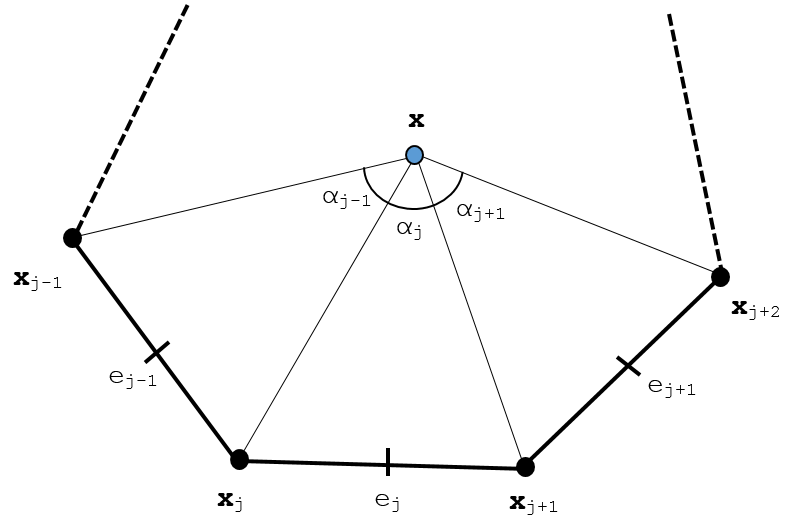
\includegraphics[width=0.65\textwidth]{figures/sec_BF/ref_polygon.png}
\caption{Arbitrary polygon with geometric properties used for 2D basis function generation.}
\label{fig::BF_2D_ref_polygon}
\end{figure}

In this dissertation, all 1st-order, two-dimensional basis functions for an element $K$ will obey the properties for barycentric coordinates. They will form a {\em partition of unity},

\begin{equation}
\sum_{i=1}^{N_K} b_i (\vec{x})  =  1;
\label{eq::BF_linear_interp_partition}
\end{equation}

\noindent coordinate interpolation will result from an {\em affine combination} of the vertices,

\begin{equation}
\sum_{i=1}^{N_K} b_i(\vec{x}) \vec{x}_i  =  \vec{x};
\label{eq::BF_linear_interp_affine}
\end{equation}

\noindent and they will satisfy the {\em Lagrange property},

\begin{equation}
b_i (\vec{x}_j) = \delta_{ij}.
\label{eq::BF_linear_interp_lagrange}
\end{equation}

\noindent $N_K$ is again the number of spatial degrees with measure in element $K$. Using the {\em partition of unity} of Eq. (\ref{eq::BF_linear_interp_partition}), we can rewrite Eqs. (\ref{eq::BF_linear_interp_partition}-\ref{eq::BF_linear_interp_affine}) into a separate, compact, vectorized form for completeness

\begin{equation}
\sum_{i=1}^{N_K}  b_i (\vec{x}) \vec{c}_{i,1}(\vec{x}) = \vec{q}_1 ,
\label{eq::BF_linear_interp_req_vector}
\end{equation}

\noindent where $\vec{c}_{i,1}(\vec{x})$ and $\vec{q}_1$ are the lineary-complete constraint and equivalence terms, respectively. These terms are simply:

\begin{equation}
\vec{c}_{i,1}(\vec{x}) = \left[
\begin{array}{c}
1 \\
x_i - x \\
y_i - y
\end{array} \right]
  \qquad \text{and} \qquad \vec{q}_1 = \left[
\begin{array}{c}
1 \\
0 \\
0
\end{array} \right],
\label{eq::BF_linear_constraint_terms}
\end{equation}

\noindent respectively. Equation (\ref{eq::BF_linear_interp_req_vector}) states that our interpolation functions (the basis functions) can exactly reproduce polynomial functions up to order 1. This is why we state that our basis functions are linearly-complete. However, we will not restrict our $N_K$ basis functions to be polynomials. In fact, of the basis functions that we will use, only the PWL coordinates are formed by combinations of polynomial functions.

%%%%%%%%%%%%%%%%%%%%%%%%%%%%%%%%%%%%%%%%%%%%%%%%%%%
%%%   SubSection - Linear
\subsection{Traditional Linear Basis Functions - $\mathbb{P}_{1}$ and $\mathbb{Q}_{1}$ Spaces}
\label{sec::BF_2DLinear_LDandBLD}

Before presenting basis function sets applicable to polygonal finite elements, we first provide two common basis functions that are exact on triangles and convex quadrilaterals: the $\mathbb{P}_{1}$ and $\mathbb{Q}_{1}$ spaces, respectively. 

\begin{equation}
\label{eq::2D_lin_basis_functions}
\begin{aligned}
	b_1(r,s) & = 1-r-s \\
	b_2(r,s) & = r \\
	b_3(r,s) & = s 
\end{aligned}
\end{equation}

\noindent 

and

\begin{equation}
\label{eq::BiL_basis_functions}
\begin{aligned}
	b_1(r,s) & = (1-r)(1-s) \\
	b_2(r,s) & = r(1-s) \\
	b_3(r,s) & = rs \\
	b_4(r,s) & = (1-r)s
\end{aligned}
\end{equation}


%%%%%%%%%%%%%%%%%%%%%%%%%%%%%%%%%%%%%%%%%%%%%%%%%%%
%%%   SubSection - Wachspress
\subsection{Wachspress Rational Basis Functions}
\label{sec::BF_2DLinear_Wachspress}

\begin{equation}
\label{eq::BF_wach_BF}
b_{j}^{W} (\vec{x}) = \frac{w_j (\vec{x}) }{\sum_i w_i (\vec{x})}
\end{equation}

\noindent where the Wachspress weight function for vertex $j$, $w_j$, has the following definition:

\begin{equation}
\label{eq::BF_wach_weights}
w_j (\vec{x})  = \frac{A(\vec{x}_{j-1}, \vec{x}_{j}, \vec{x}_{j+1})}{A(\vec{x}, \vec{x}_{j-1}, \vec{x}_{j}) \, A(\vec{x}, \vec{x}_{j}, \vec{x}_{j+1})}
\end{equation}



\begin{figure}
\label{fig::2D_WACHSPRESS1_unit_square_basis_functions}
\centering
	\begin{subfigure}[b]{0.39\textwidth}
		\centering
		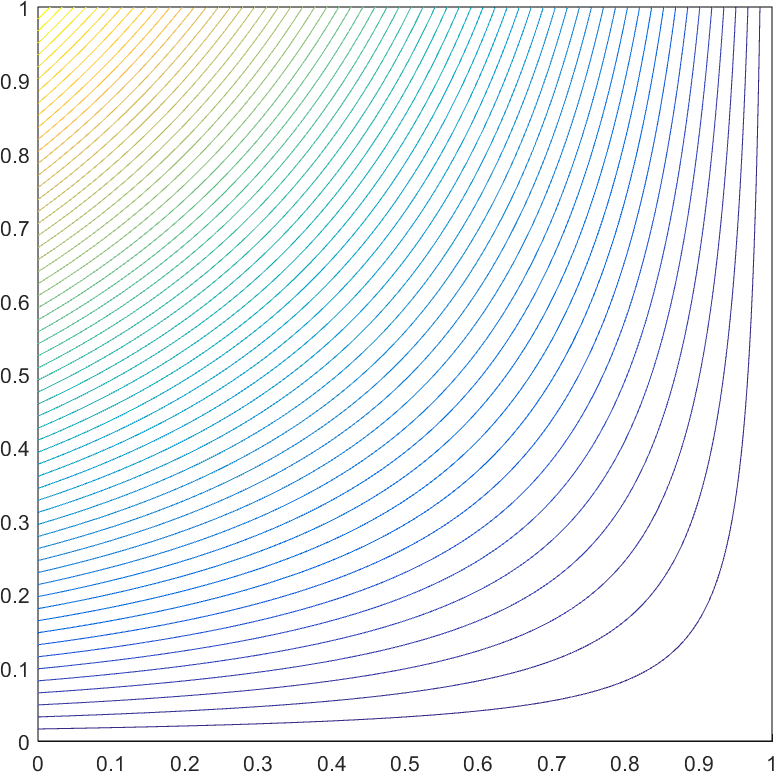
\includegraphics[width=\textwidth]{figures/sec_BF/square_WACHSPRESS1_contour_b4.png}
		\caption{}
	\end{subfigure}
	\hspace{1.5cm}
	\begin{subfigure}[b]{0.39\textwidth}
		\centering
		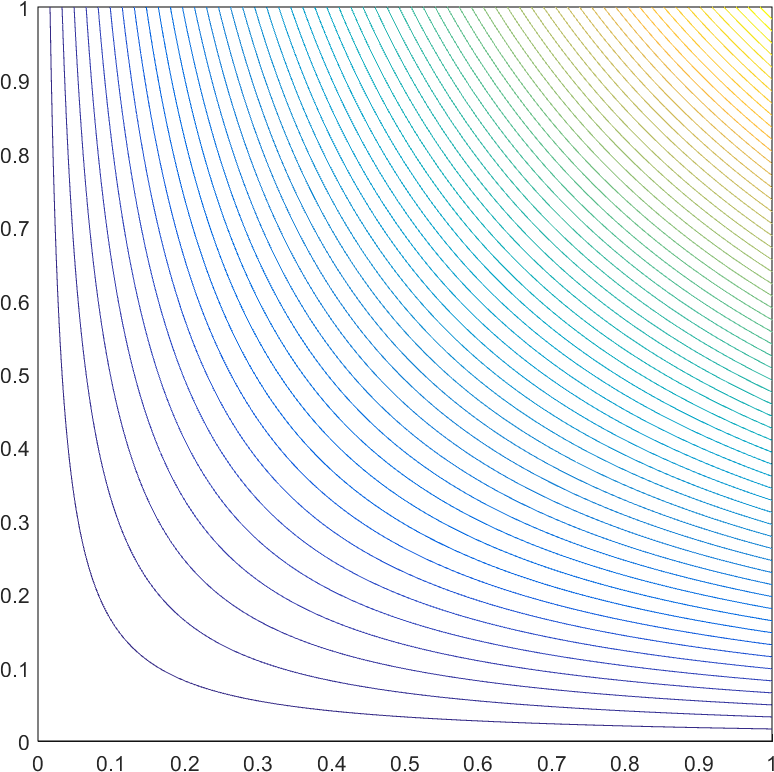
\includegraphics[width=\textwidth]{figures/sec_BF/square_WACHSPRESS1_contour_b3.png}
		\caption{}
	\end{subfigure}
	\vfill
	\begin{subfigure}[b]{0.39\textwidth}
		\centering
		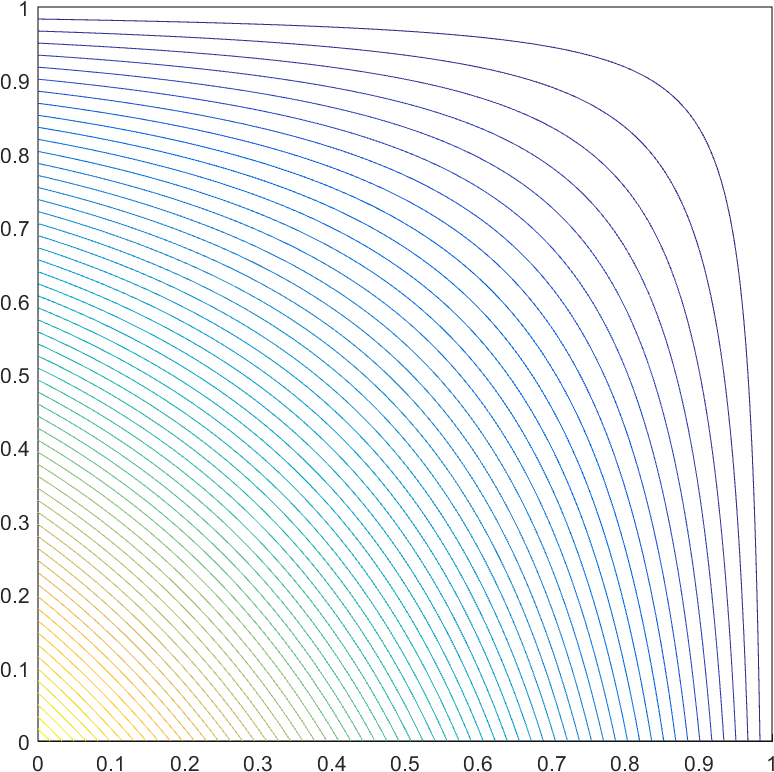
\includegraphics[width=\textwidth]{figures/sec_BF/square_WACHSPRESS1_contour_b1.png}
		\caption{}
	\end{subfigure}
	\hspace{1.5cm}
	\begin{subfigure}[b]{0.39\textwidth}
		\centering
		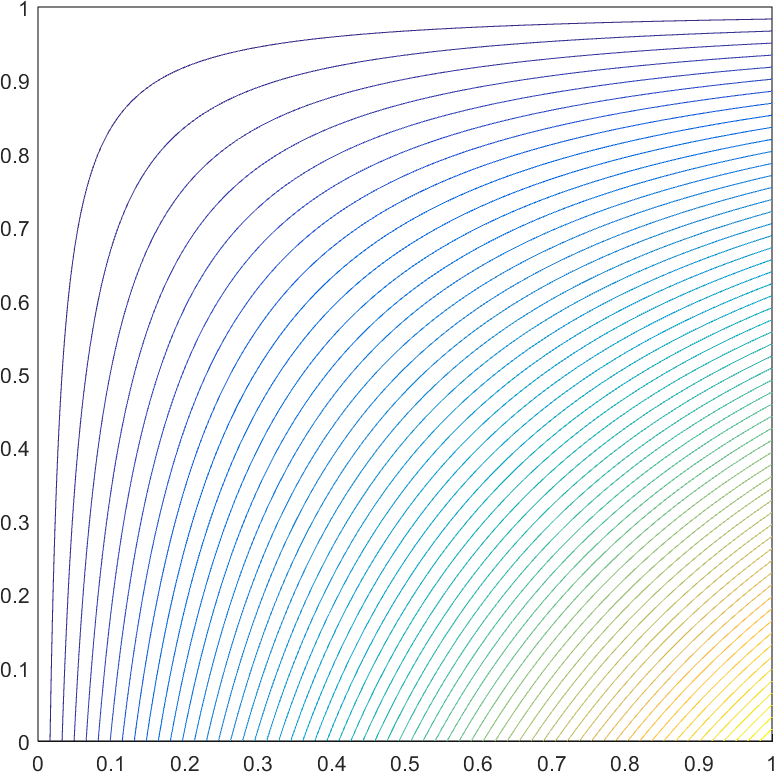
\includegraphics[width=\textwidth]{figures/sec_BF/square_WACHSPRESS1_contour_b2.png}
		\caption{}
	\end{subfigure}
\caption{Contour plots of the linear Wachspress basis functions on the unit square for the vertices located at: (a) (0,1), (b) (1,1), (c) (0,0), and (d) (1,0).}
\end{figure}

\begin{figure}
\label{fig::2D_WACHSPRESS1_deg_square_basis_functions}
\centering
	\begin{subfigure}[b]{0.39\textwidth}
		\centering
		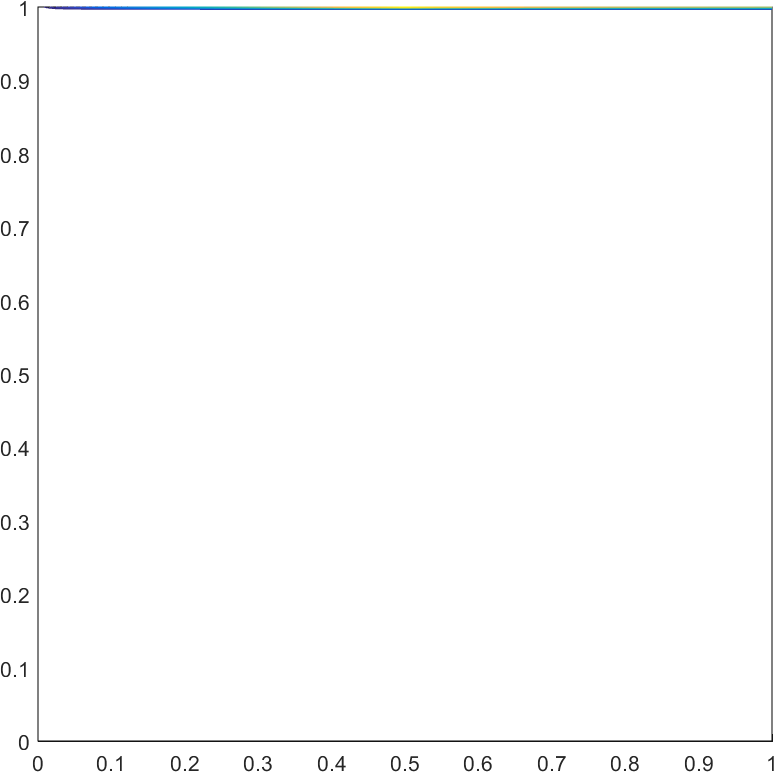
\includegraphics[width=\textwidth]{figures/sec_BF/deg_square_WACHSPRESS1_contour_b4.png}
		\caption{}
	\end{subfigure}
	\vfill
	\begin{subfigure}[b]{0.39\textwidth}
		\centering
		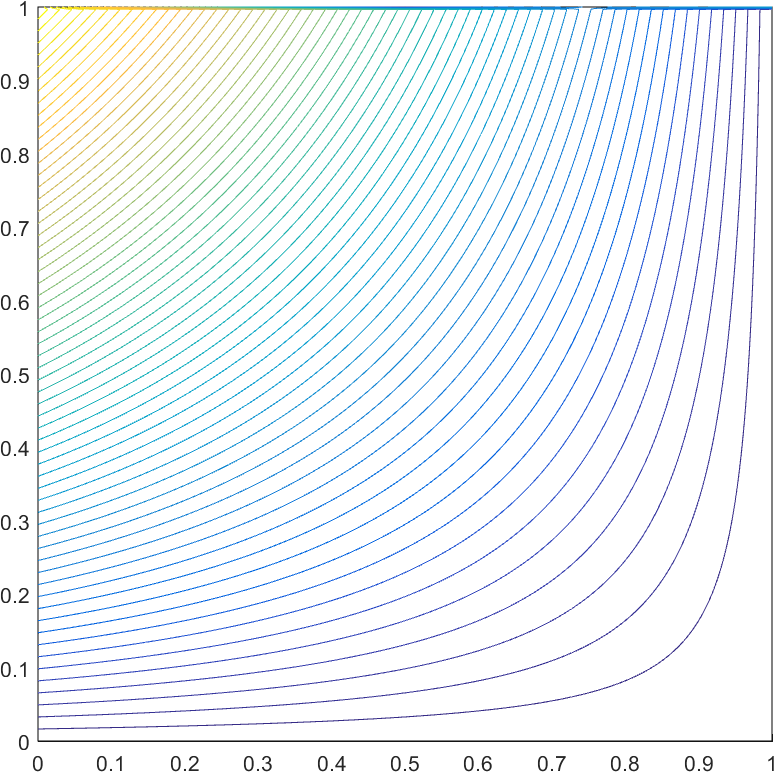
\includegraphics[width=\textwidth]{figures/sec_BF/deg_square_WACHSPRESS1_contour_b5.png}
		\caption{}
	\end{subfigure}
	\hspace{1.5cm}
	\begin{subfigure}[b]{0.39\textwidth}
		\centering
		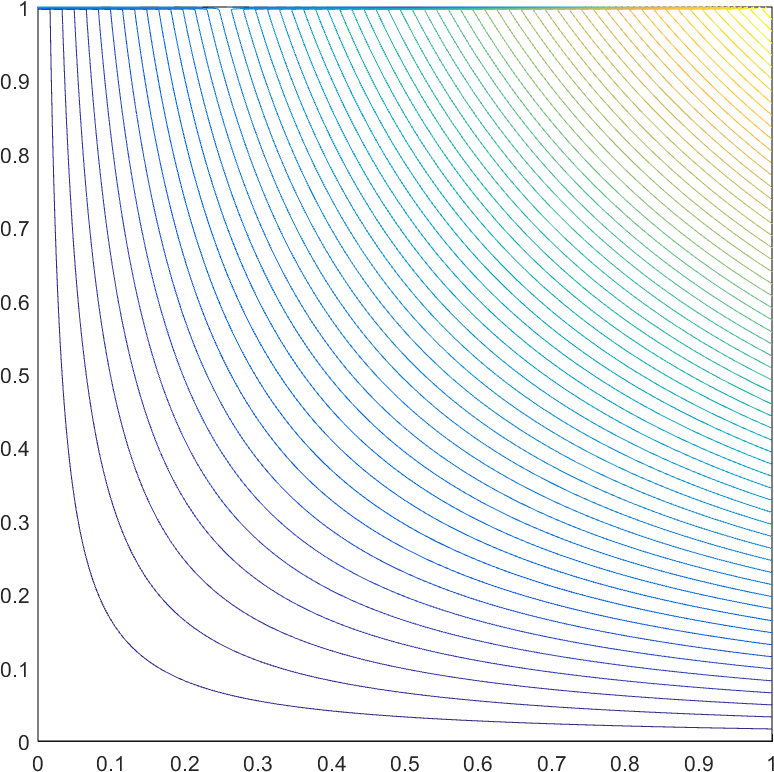
\includegraphics[width=\textwidth]{figures/sec_BF/deg_square_WACHSPRESS1_contour_b3.png}
		\caption{}
	\end{subfigure}
	\vfill
	\begin{subfigure}[b]{0.39\textwidth}
		\centering
		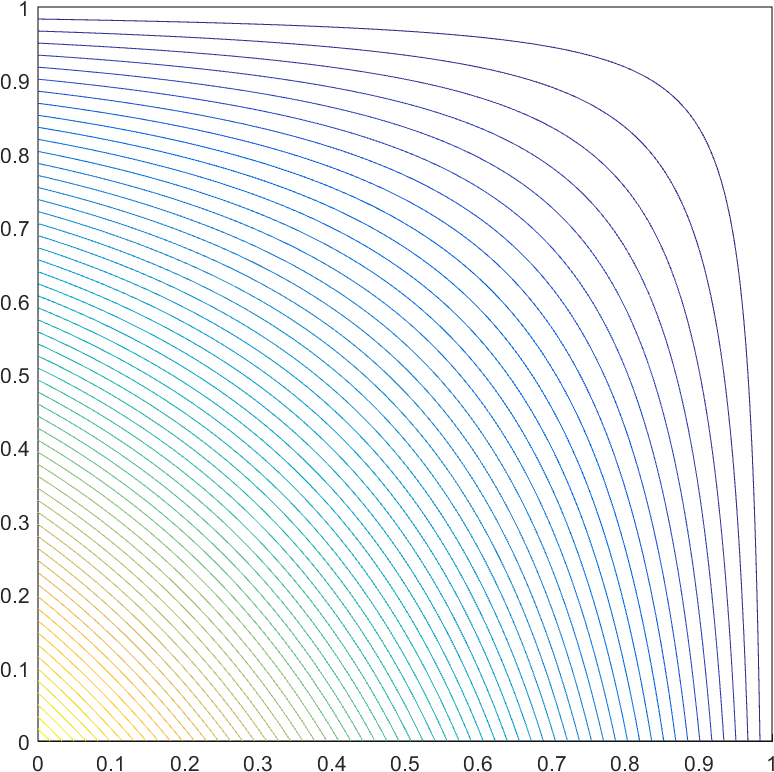
\includegraphics[width=\textwidth]{figures/sec_BF/deg_square_WACHSPRESS1_contour_b1.png}
		\caption{}
	\end{subfigure}
	\hspace{1.5cm}
	\begin{subfigure}[b]{0.39\textwidth}
		\centering
		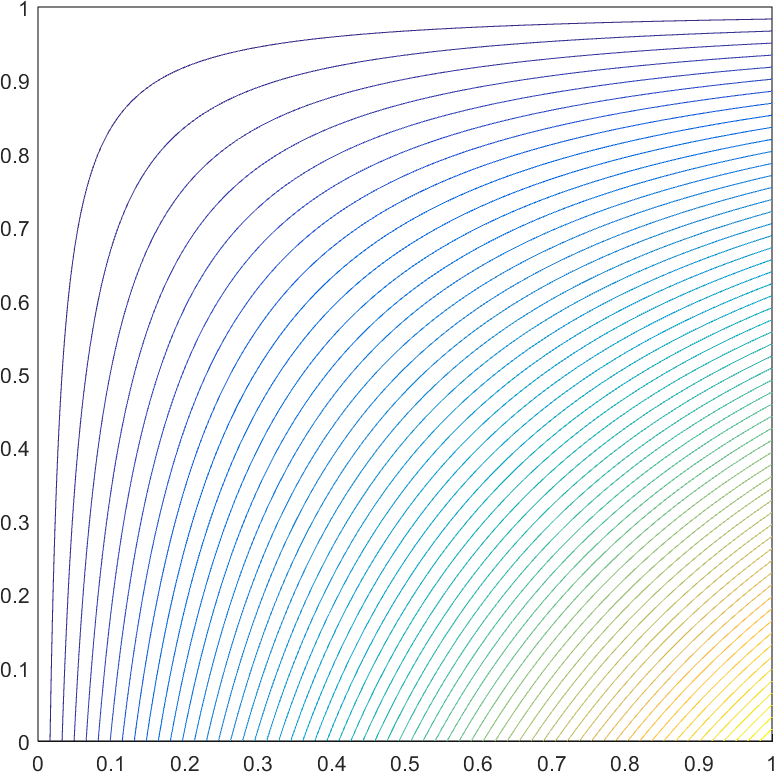
\includegraphics[width=\textwidth]{figures/sec_BF/deg_square_WACHSPRESS1_contour_b2.png}
		\caption{}
	\end{subfigure}
\caption{Contour plots of the linear Wachspress basis functions on the degnerate pentagon for the vertices located at: (a) (1/2,1), (b) (0,1), (c) (1,1), (d) (0,0), and (e) (1,0).}
\end{figure}

%%%%%%%%%%%%%%%%%%%%%%%%%%%%%%%%%%%%%%%%%%%%%%%%%%%
%%%   SubSection - PWL
\subsection{Piecewise Linear (PWL) Basis Functions}
\label{sec::BF_2DLinear_PWL}

\begin{equation}
\label{eq::PWL_2D}
	b_j^{PWL} (x,y) = t_j (x,y) + \alpha_j^K t_c (x,y)
\end{equation}

\noindent $t_j$ is the standard 2D linear function with unity at vertex $j$ that linearly decreases to zero to the cell center and each adjoining vertex. $t_c$ is the 2D cell ``tent'' function which is unity at the cell center and linearly decreases to zero to each cell vertex. $\alpha_{j}^{K}$ is the weight parameter for vertex $j$ in cell $K$. 

\begin{figure}
\label{fig::2D_PWLD1_unit_square_basis_functions}
\centering
	\begin{subfigure}[b]{0.39\textwidth}
		\centering
		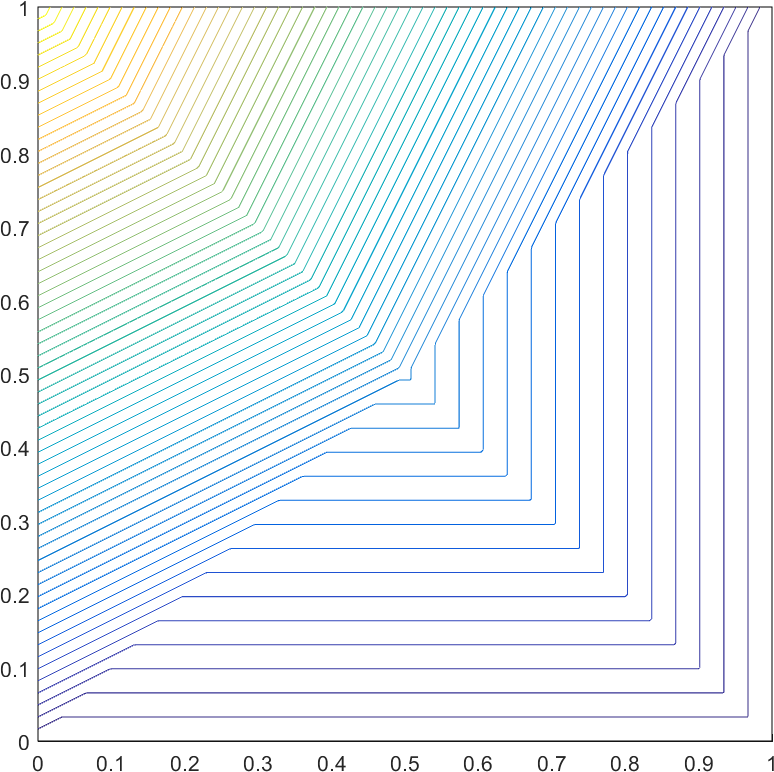
\includegraphics[width=\textwidth]{figures/sec_BF/square_PWLD1_contour_b4.png}
		\caption{}
	\end{subfigure}
	\hspace{1.5cm}
	\begin{subfigure}[b]{0.39\textwidth}
		\centering
		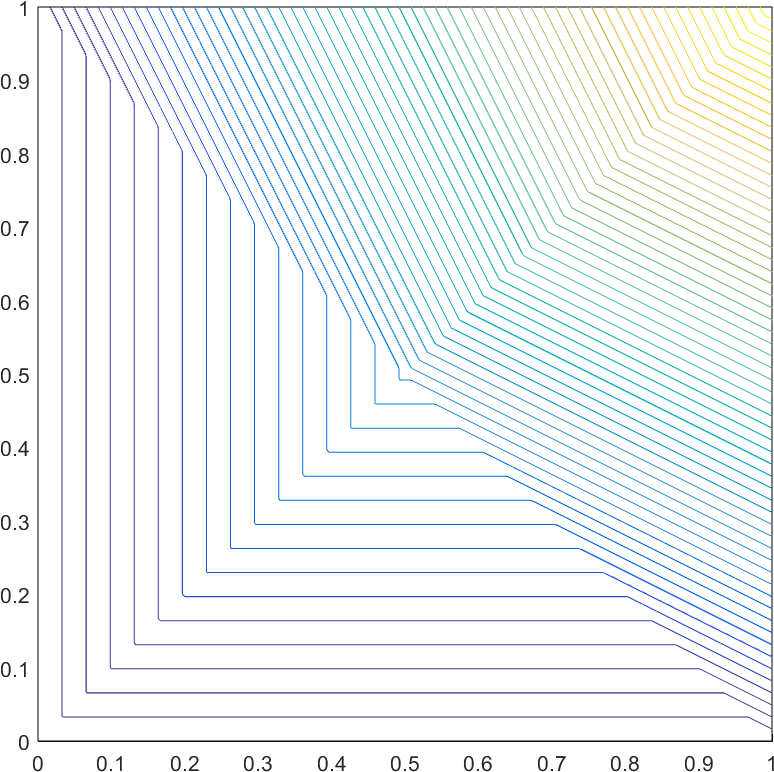
\includegraphics[width=\textwidth]{figures/sec_BF/square_PWLD1_contour_b3.png}
		\caption{}
	\end{subfigure}
	\vfill
	\begin{subfigure}[b]{0.39\textwidth}
		\centering
		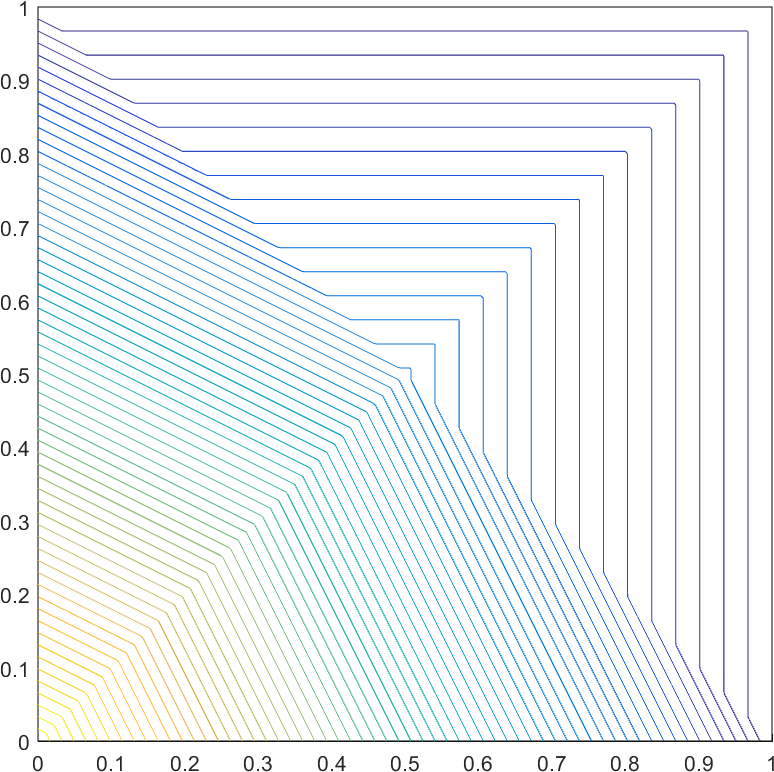
\includegraphics[width=\textwidth]{figures/sec_BF/square_PWLD1_contour_b1.png}
		\caption{}
	\end{subfigure}
	\hspace{1.5cm}
	\begin{subfigure}[b]{0.39\textwidth}
		\centering
		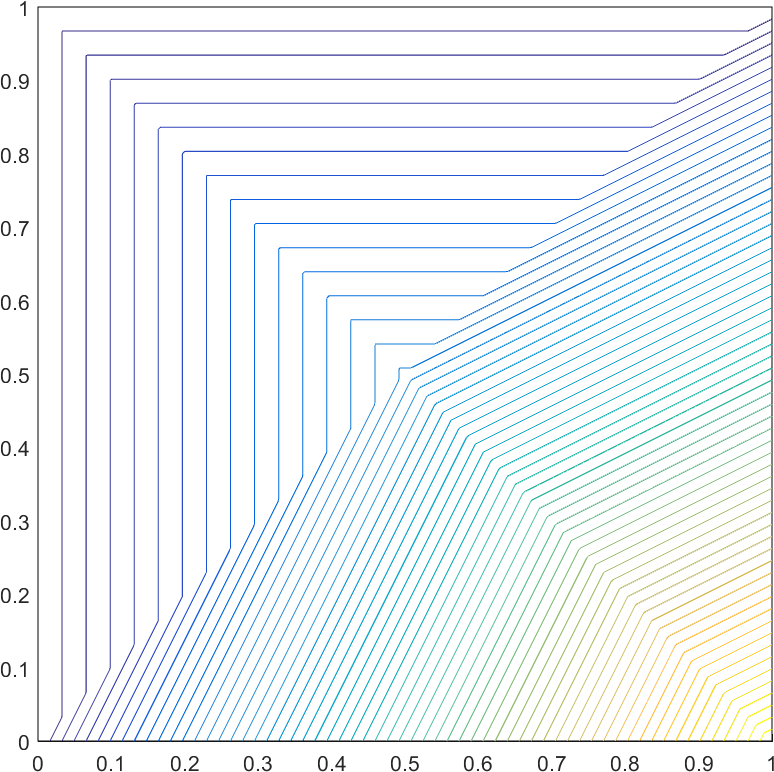
\includegraphics[width=\textwidth]{figures/sec_BF/square_PWLD1_contour_b2.png}
		\caption{}
	\end{subfigure}
\caption{Contour plots of the linear PWL basis functions on the unit square for the vertices located at: (a) (0,1), (b) (1,1), (c) (0,0), and (d) (1,0).}
\end{figure}

\begin{figure}
\label{fig::2D_PWLD1_deg_square_basis_functions}
\centering
	\begin{subfigure}[b]{0.39\textwidth}
		\centering
		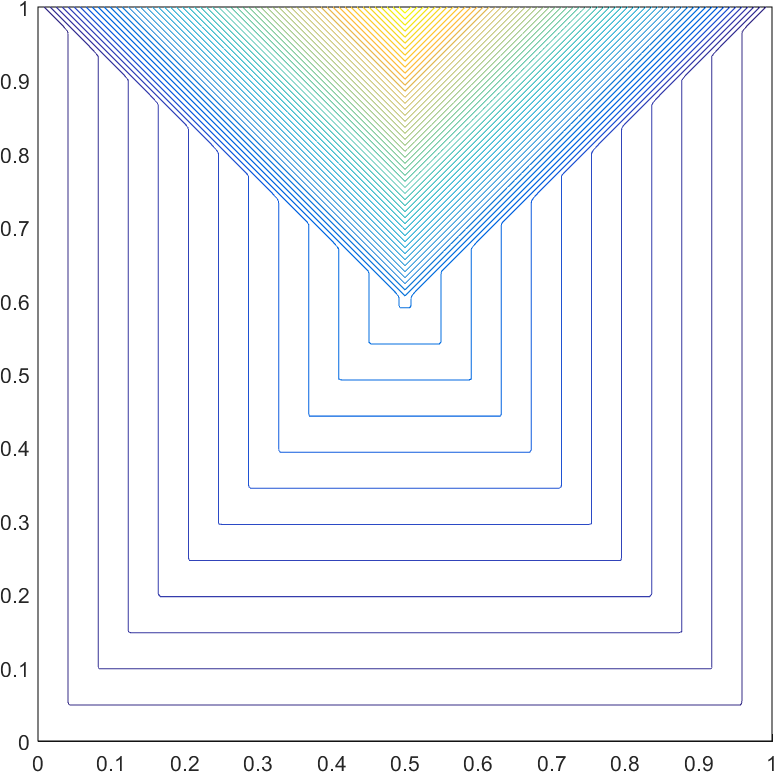
\includegraphics[width=\textwidth]{figures/sec_BF/deg_square_PWLD1_contour_b4.png}
		\caption{}
	\end{subfigure}
	\vfill
	\begin{subfigure}[b]{0.39\textwidth}
		\centering
		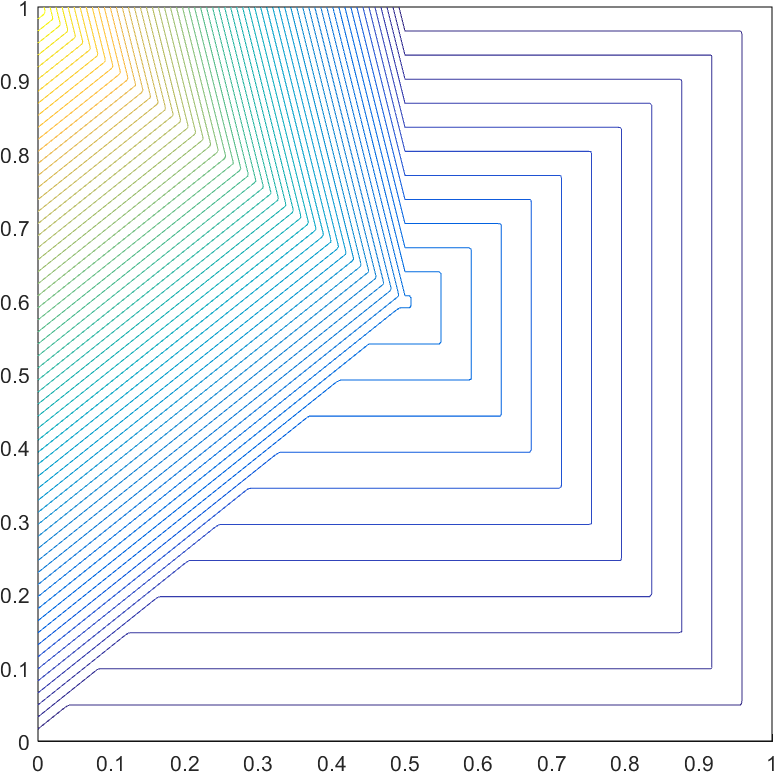
\includegraphics[width=\textwidth]{figures/sec_BF/deg_square_PWLD1_contour_b5.png}
		\caption{}
	\end{subfigure}
	\hspace{1.5cm}
	\begin{subfigure}[b]{0.39\textwidth}
		\centering
		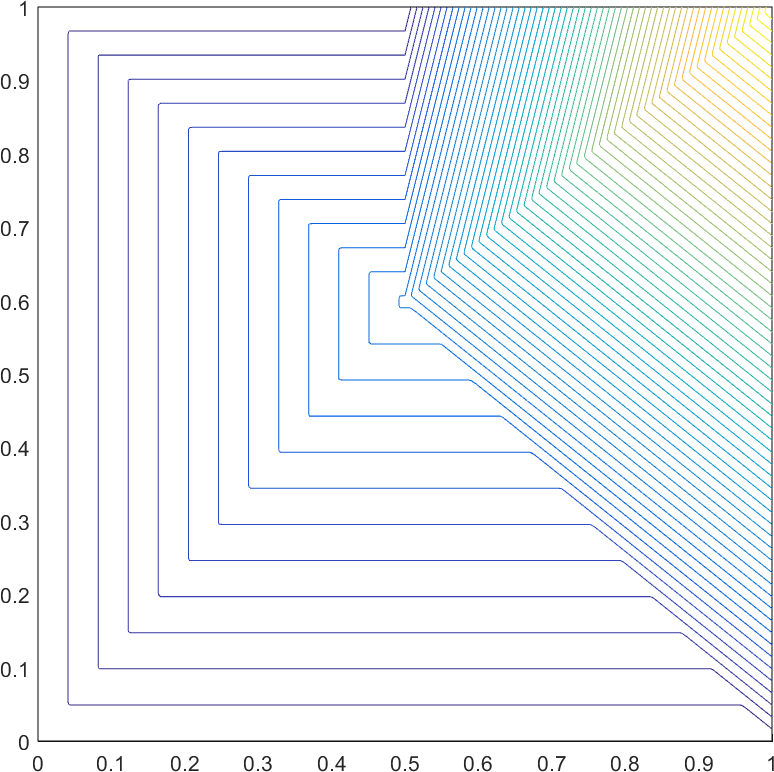
\includegraphics[width=\textwidth]{figures/sec_BF/deg_square_PWLD1_contour_b3.png}
		\caption{}
	\end{subfigure}
	\vfill
	\begin{subfigure}[b]{0.39\textwidth}
		\centering
		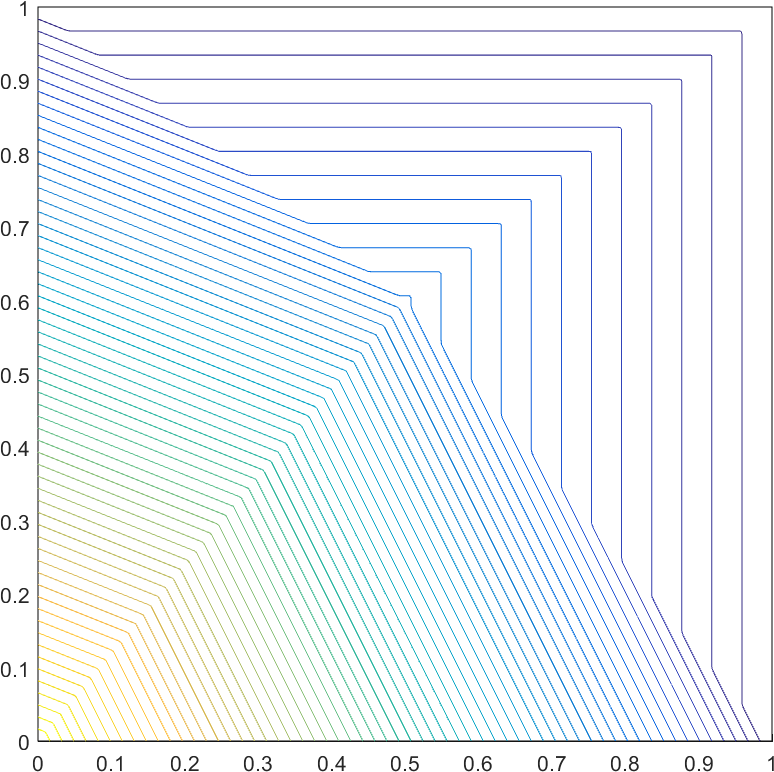
\includegraphics[width=\textwidth]{figures/sec_BF/deg_square_PWLD1_contour_b1.png}
		\caption{}
	\end{subfigure}
	\hspace{1.5cm}
	\begin{subfigure}[b]{0.39\textwidth}
		\centering
		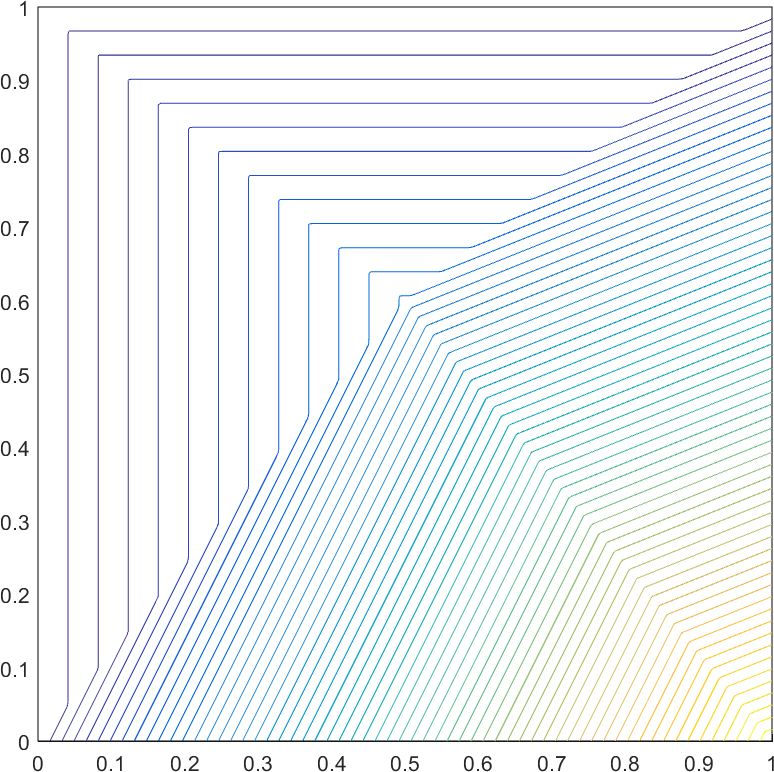
\includegraphics[width=\textwidth]{figures/sec_BF/deg_square_PWLD1_contour_b2.png}
		\caption{}
	\end{subfigure}
\caption{Contour plots of the linear PWL basis functions on the degnerate pentagon for the vertices located at: (a) (1/2,1), (b) (0,1), (c) (1,1), (d) (0,0), and (e) (1,0).}
\end{figure}

\begin{figure}
\label{fig::2D_PWLD1_Ldom_basis_functions}
\centering
	\begin{subfigure}[b]{0.39\textwidth}
		\centering
		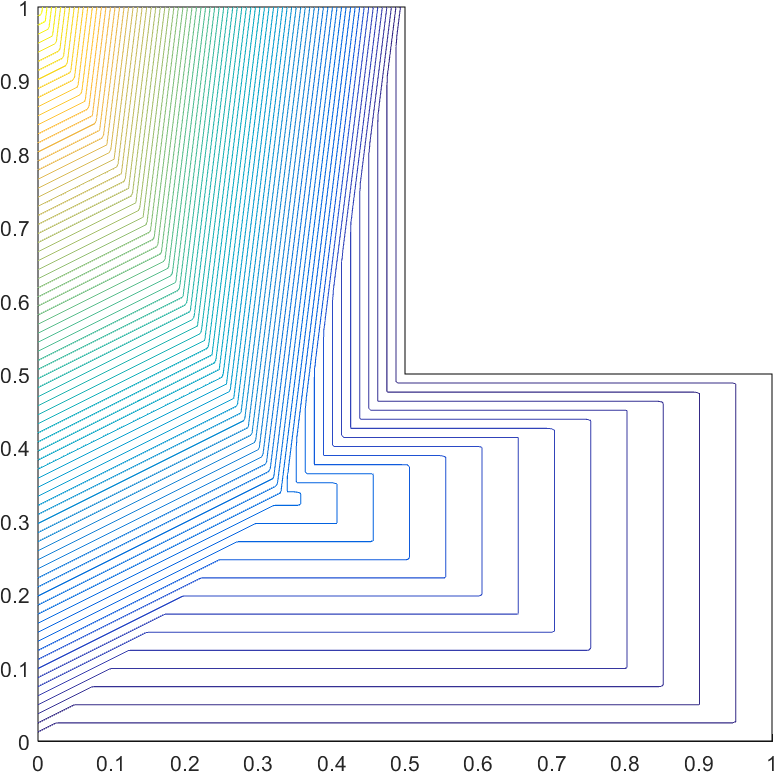
\includegraphics[width=\textwidth]{figures/sec_BF/L-domain_PWLD1_contour_b6.png}
		\caption{}
	\end{subfigure}
	\hspace{1.5cm}
	\begin{subfigure}[b]{0.39\textwidth}
		\centering
		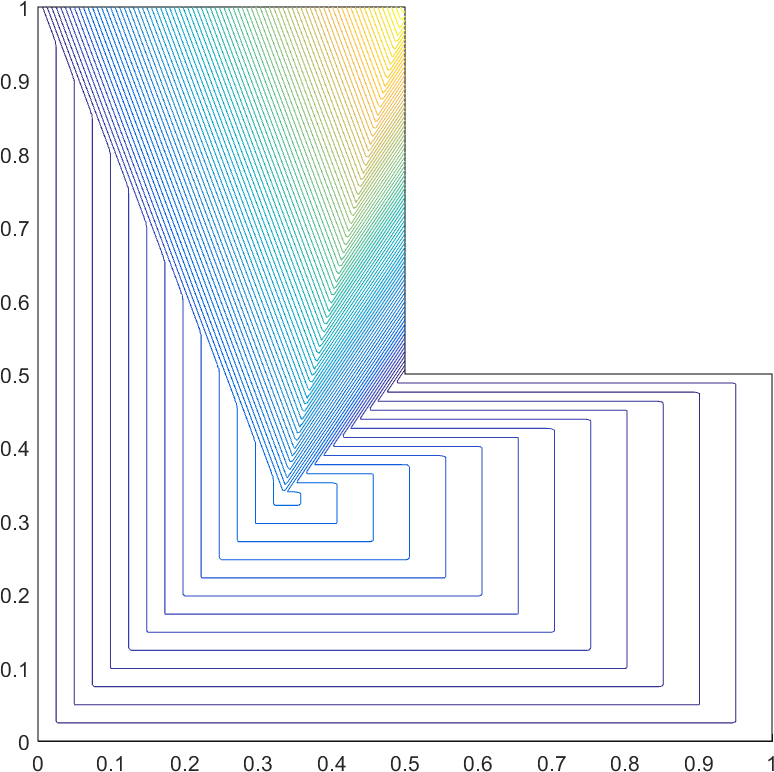
\includegraphics[width=\textwidth]{figures/sec_BF/L-domain_PWLD1_contour_b5.png}
		\caption{}
	\end{subfigure}
	\vfill
	\begin{subfigure}[b]{0.39\textwidth}
		\centering
		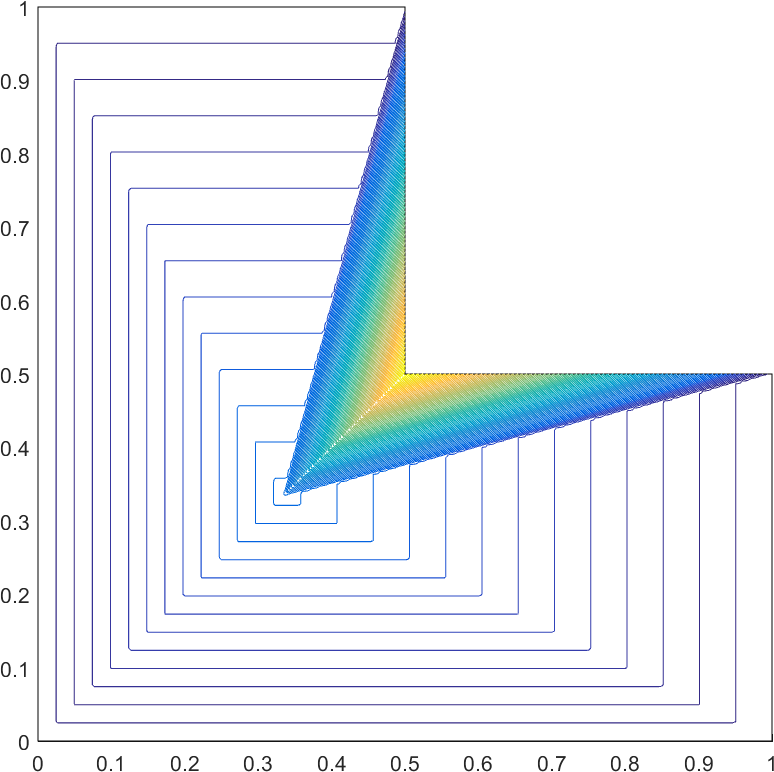
\includegraphics[width=\textwidth]{figures/sec_BF/L-domain_PWLD1_contour_b4.png}
		\caption{}
	\end{subfigure}
	\hspace{1.5cm}
	\begin{subfigure}[b]{0.39\textwidth}
		\centering
		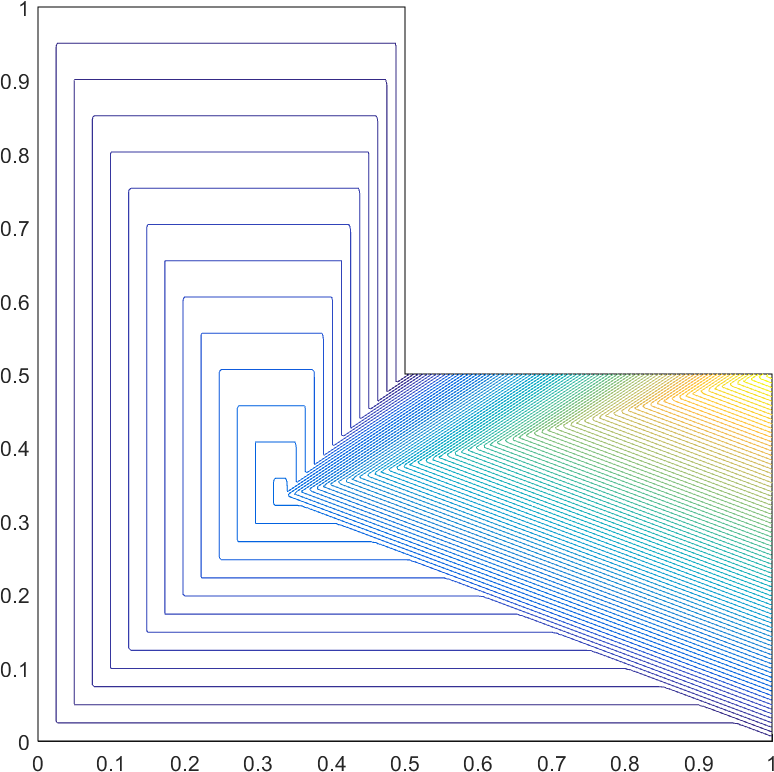
\includegraphics[width=\textwidth]{figures/sec_BF/L-domain_PWLD1_contour_b3.png}
		\caption{}
	\end{subfigure}
	\vfill
	\begin{subfigure}[b]{0.39\textwidth}
		\centering
		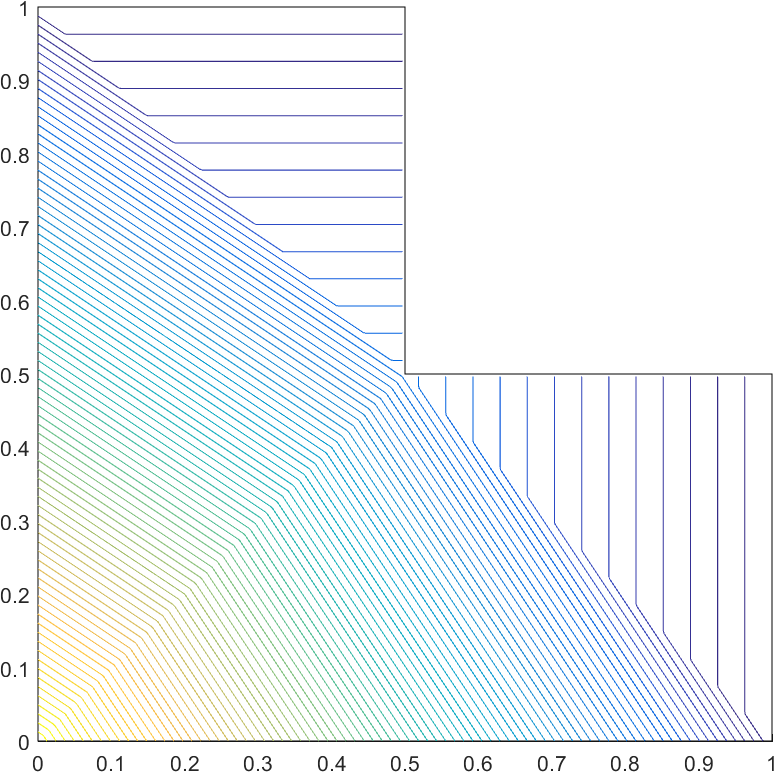
\includegraphics[width=\textwidth]{figures/sec_BF/L-domain_PWLD1_contour_b1.png}
		\caption{}
	\end{subfigure}
	\hspace{1.5cm}
	\begin{subfigure}[b]{0.39\textwidth}
		\centering
		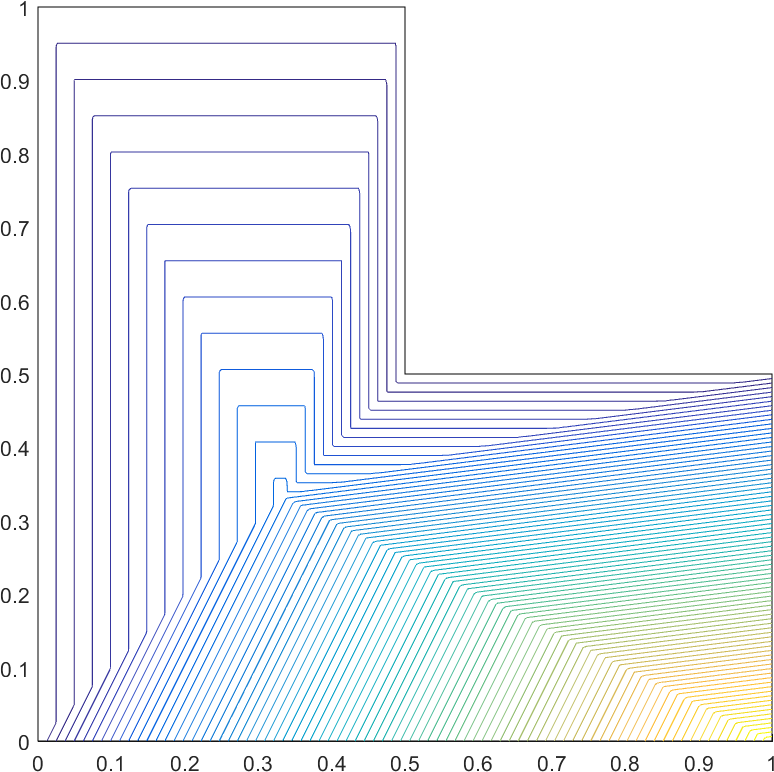
\includegraphics[width=\textwidth]{figures/sec_BF/L-domain_PWLD1_contour_b2.png}
		\caption{}
	\end{subfigure}
\caption{Contour plots of the linear PWL basis functions on the L-shaped domain for the vertices located at: (a) (0,1), (b) (1/2,1), (c) (1/2,1/2), (d) (1,1/2), (e) (0,0), and (f) (1,0).}
\end{figure}

%%%%%%%%%%%%%%%%%%%%%%%%%%%%%%%%%%%%%%%%%%%%%%%%%%%
%%%   SubSection - Mean Value
\subsection{Mean Value Basis Functions}
\label{sec::BF_2DLinear_MV}

At this point, we now introduce the first new polygonal basis set for use with the transport equation: the {\em mean value coordinates} (MV) developed by Floater \cite{floater2003mean,hormann2006mean}. The original motivation behind the MV coordinates was to approximate harmonic maps on a polygon by a set of piecewise linear maps over a triangulation of the polygon for use in computer aided graphic design.

\begin{equation}
\label{eq::BF_MV_laplace}
\nabla^2 u = 0 ,
\end{equation}

\noindent with $u(\vec{r}) = u_0$ constituting a piecewise linear function 

\begin{equation}
\label{eq::BF_MV_BF}
b_{j}^{MV} (\vec{x}) = \frac{w_j (\vec{x}) }{\sum_i w_i (\vec{x})}
\end{equation}

\noindent where the mean value weight function for vertex $j$, $w_j$, has the following definition:

\begin{equation}
\label{eq::BF_MV_weights}
w_j (\vec{x})  = \frac{\tan(\alpha_{j-1} / 2) + \tan(\alpha_j / 2)}{|\vec{x}_j - \vec{x}|}
\end{equation}

\begin{figure}
\label{fig::2D_MV1_unit_square_basis_functions}
\centering
	\begin{subfigure}[b]{0.39\textwidth}
		\centering
		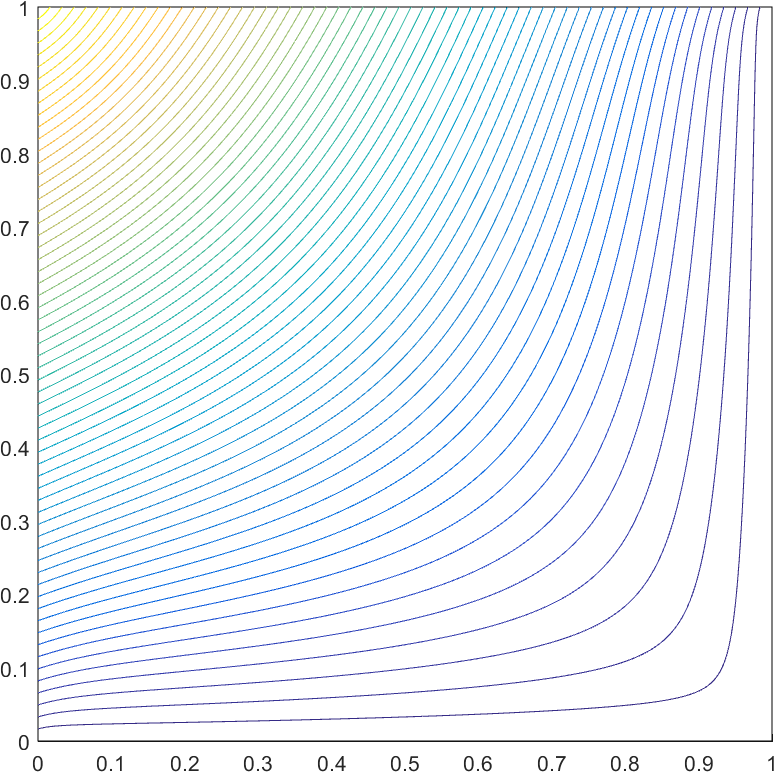
\includegraphics[width=\textwidth]{figures/sec_BF/square_MV1_contour_b4.png}
		\caption{}
	\end{subfigure}
	\hspace{1.5cm}
	\begin{subfigure}[b]{0.39\textwidth}
		\centering
		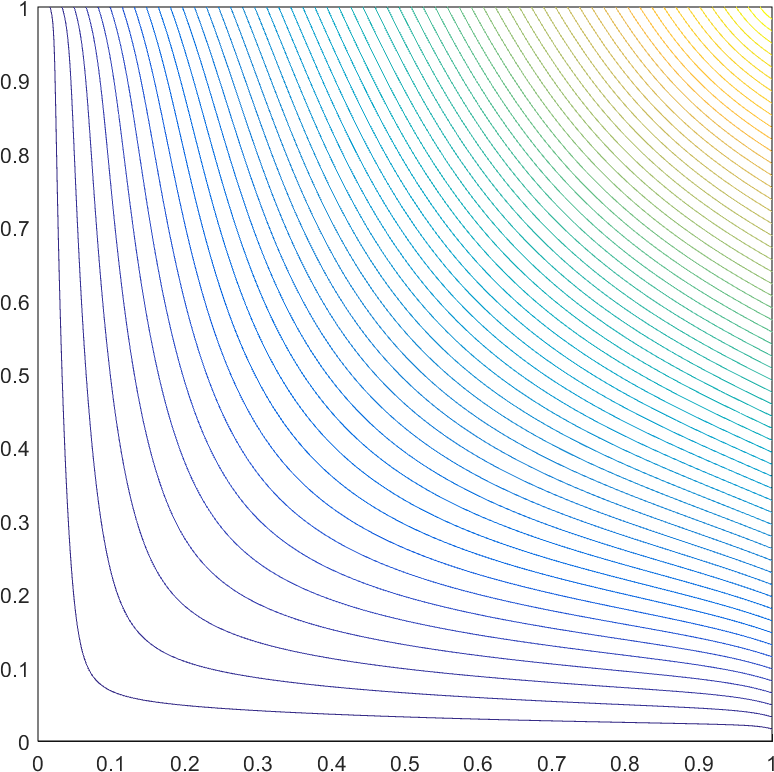
\includegraphics[width=\textwidth]{figures/sec_BF/square_MV1_contour_b3.png}
		\caption{}
	\end{subfigure}
	\vfill
	\begin{subfigure}[b]{0.39\textwidth}
		\centering
		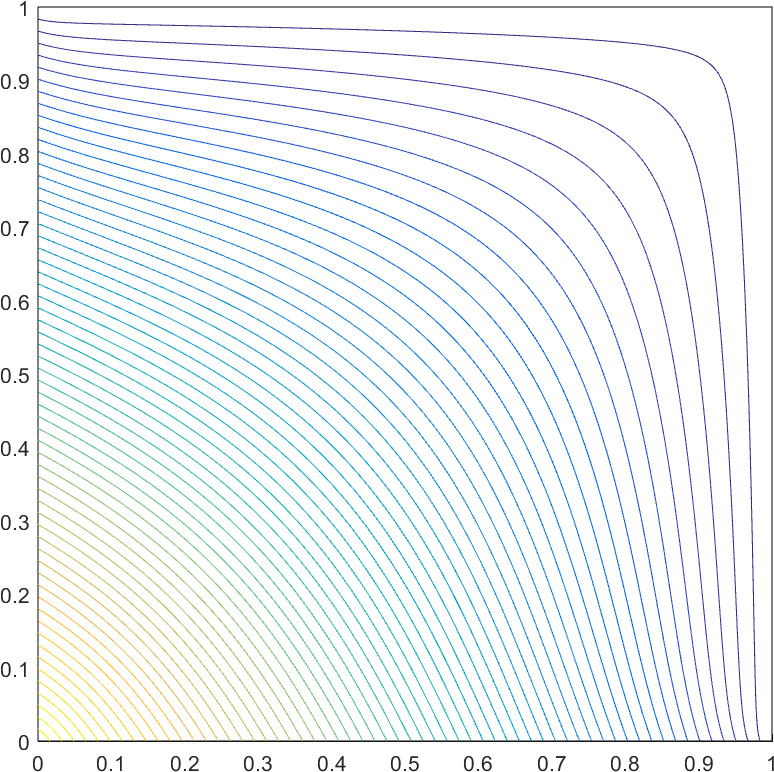
\includegraphics[width=\textwidth]{figures/sec_BF/square_MV1_contour_b1.png}
		\caption{}
	\end{subfigure}
	\hspace{1.5cm}
	\begin{subfigure}[b]{0.39\textwidth}
		\centering
		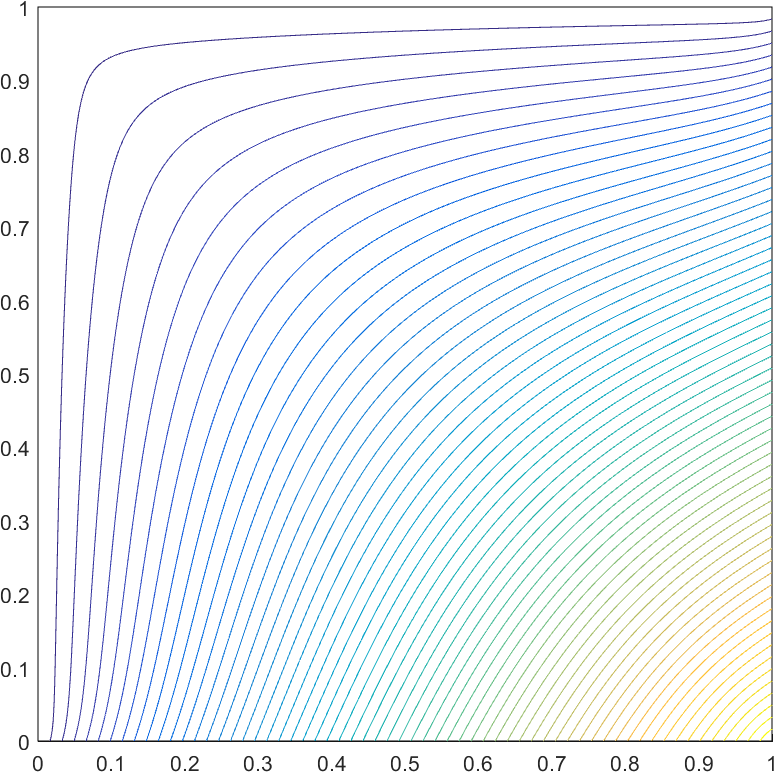
\includegraphics[width=\textwidth]{figures/sec_BF/square_MV1_contour_b2.png}
		\caption{}
	\end{subfigure}
\caption{Contour plots of the linear mean value basis functions on the unit square for the vertices located at: (a) (0,1), (b) (1,1), (c) (0,0), and (d) (1,0).}
\end{figure}

\begin{figure}
\label{fig::2D_MV1_deg_square_basis_functions}
\centering
	\begin{subfigure}[b]{0.39\textwidth}
		\centering
		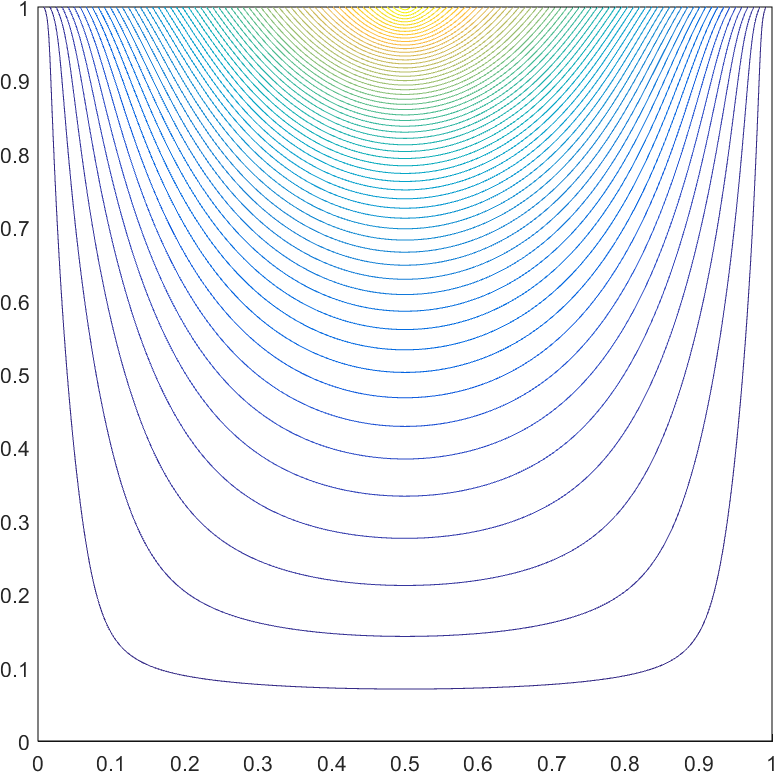
\includegraphics[width=\textwidth]{figures/sec_BF/deg_square_MV1_contour_b4.png}
		\caption{}
	\end{subfigure}
	\vfill
	\begin{subfigure}[b]{0.39\textwidth}
		\centering
		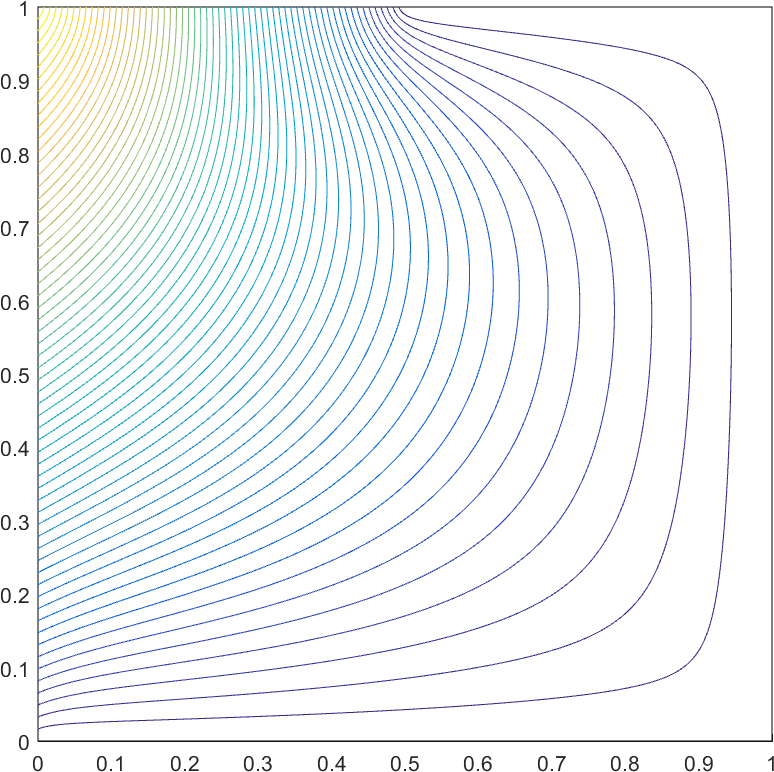
\includegraphics[width=\textwidth]{figures/sec_BF/deg_square_MV1_contour_b5.png}
		\caption{}
	\end{subfigure}
	\hspace{1.5cm}
	\begin{subfigure}[b]{0.39\textwidth}
		\centering
		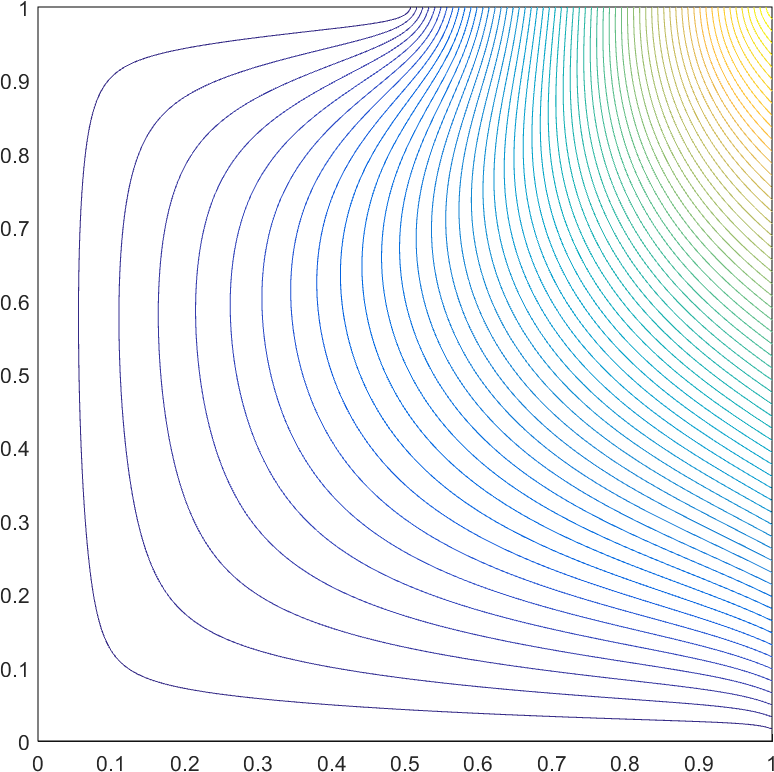
\includegraphics[width=\textwidth]{figures/sec_BF/deg_square_MV1_contour_b3.png}
		\caption{}
	\end{subfigure}
	\vfill
	\begin{subfigure}[b]{0.39\textwidth}
		\centering
		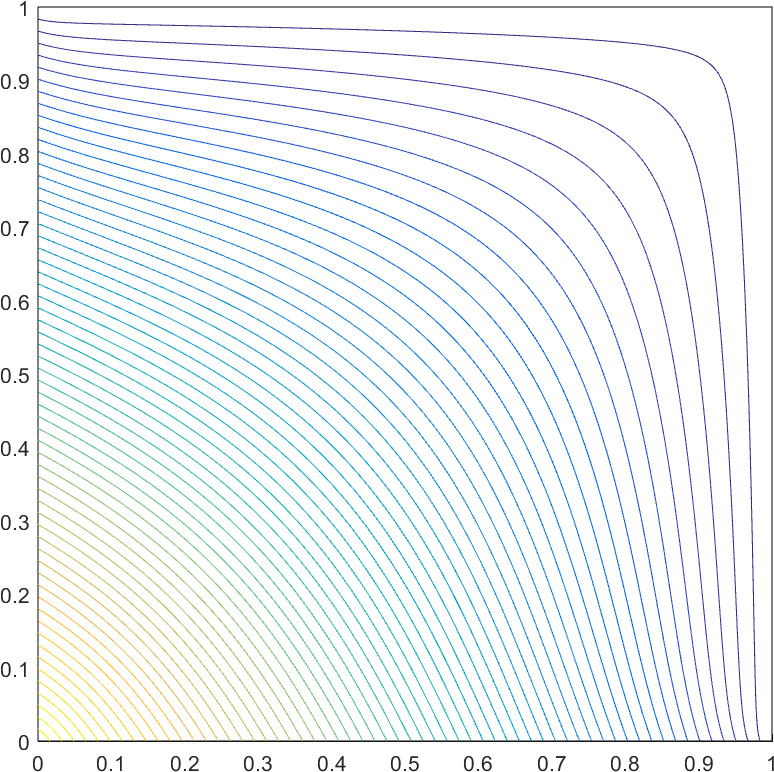
\includegraphics[width=\textwidth]{figures/sec_BF/deg_square_MV1_contour_b1.png}
		\caption{}
	\end{subfigure}
	\hspace{1.5cm}
	\begin{subfigure}[b]{0.39\textwidth}
		\centering
		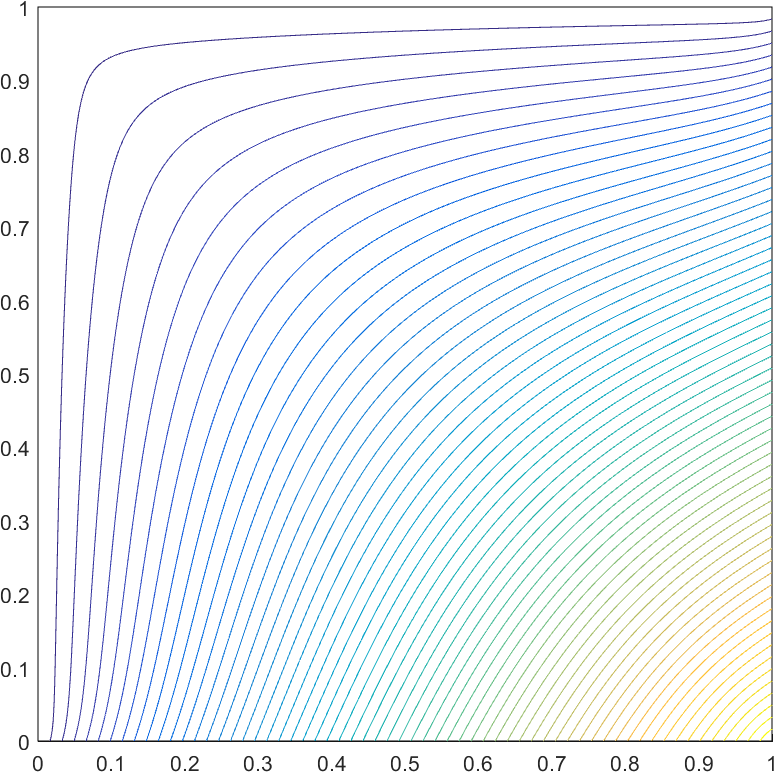
\includegraphics[width=\textwidth]{figures/sec_BF/deg_square_MV1_contour_b2.png}
		\caption{}
	\end{subfigure}
\caption{Contour plots of the linear mean value basis functions on the degnerate pentagon for the vertices located at: (a) (1/2,1), (b) (0,1), (c) (1,1), (d) (0,0), and (e) (1,0).}
\end{figure}

\begin{figure}
\label{fig::2D_MV1_Ldom_basis_functions}
\centering
	\begin{subfigure}[b]{0.39\textwidth}
		\centering
		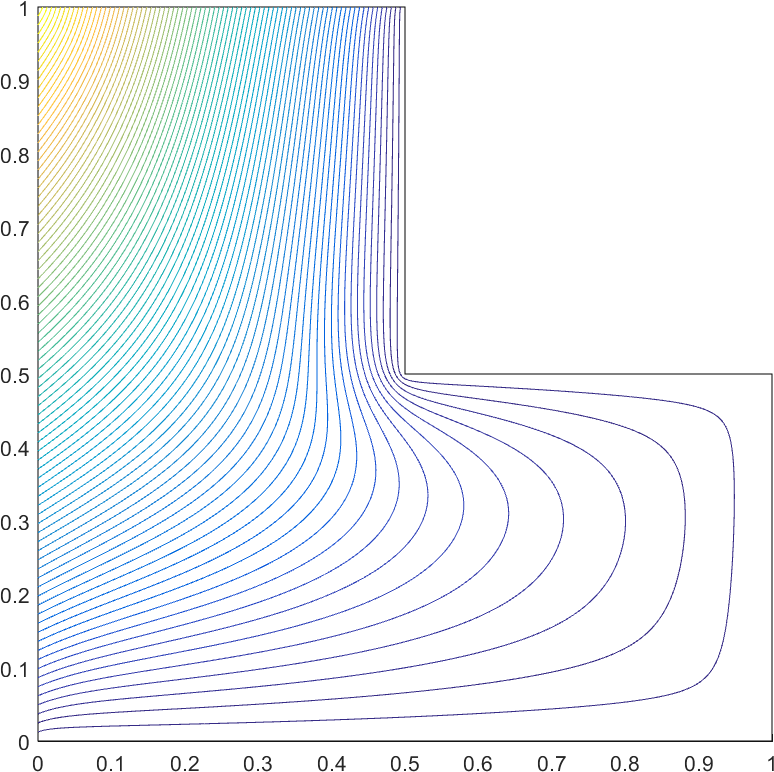
\includegraphics[width=\textwidth]{figures/sec_BF/L-domain_MV1_contour_b6.png}
		\caption{}
	\end{subfigure}
	\hspace{1.5cm}
	\begin{subfigure}[b]{0.39\textwidth}
		\centering
		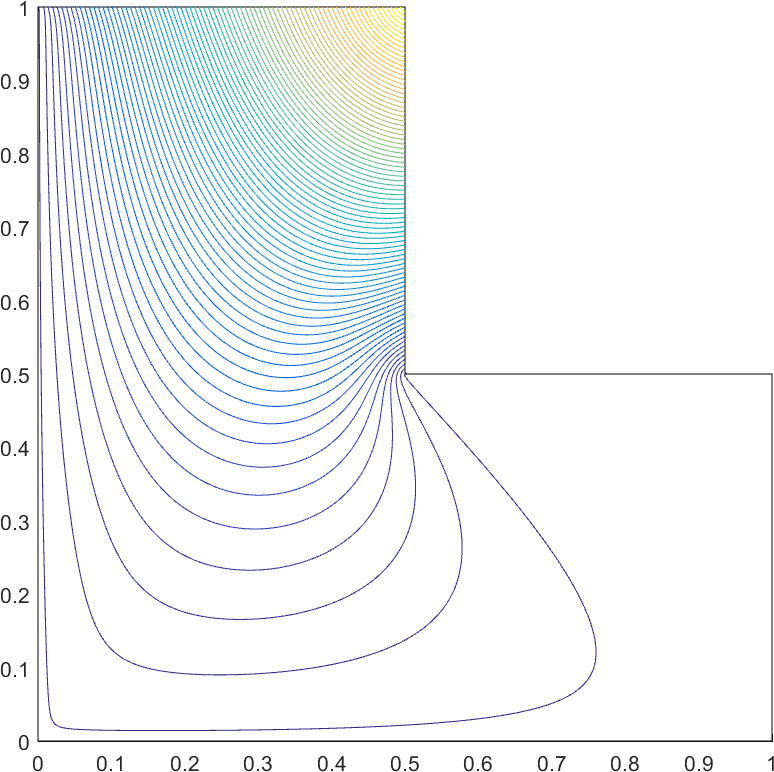
\includegraphics[width=\textwidth]{figures/sec_BF/L-domain_MV1_contour_b5.png}
		\caption{}
	\end{subfigure}
	\vfill
	\begin{subfigure}[b]{0.39\textwidth}
		\centering
		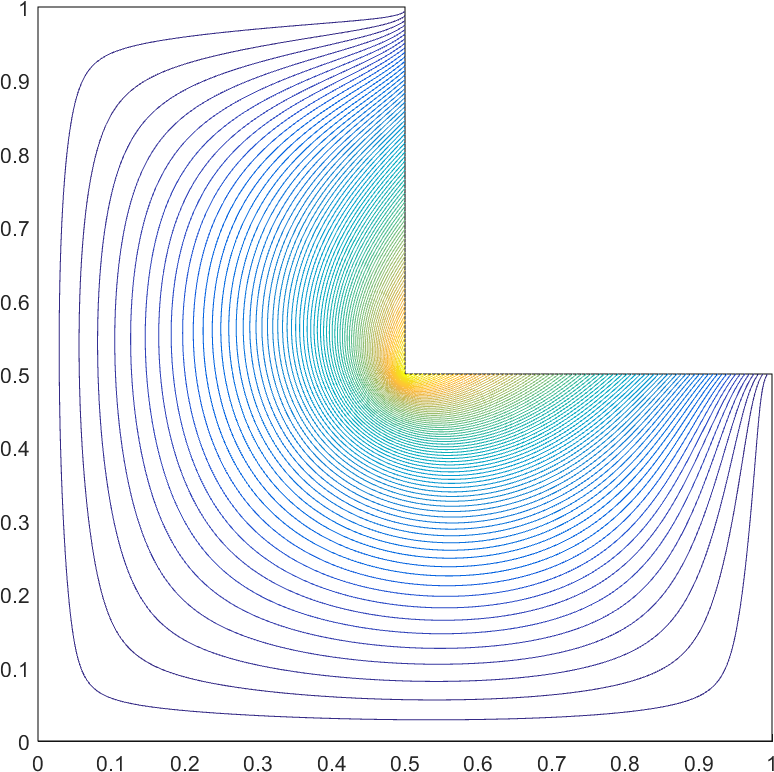
\includegraphics[width=\textwidth]{figures/sec_BF/L-domain_MV1_contour_b4.png}
		\caption{}
	\end{subfigure}
	\hspace{1.5cm}
	\begin{subfigure}[b]{0.39\textwidth}
		\centering
		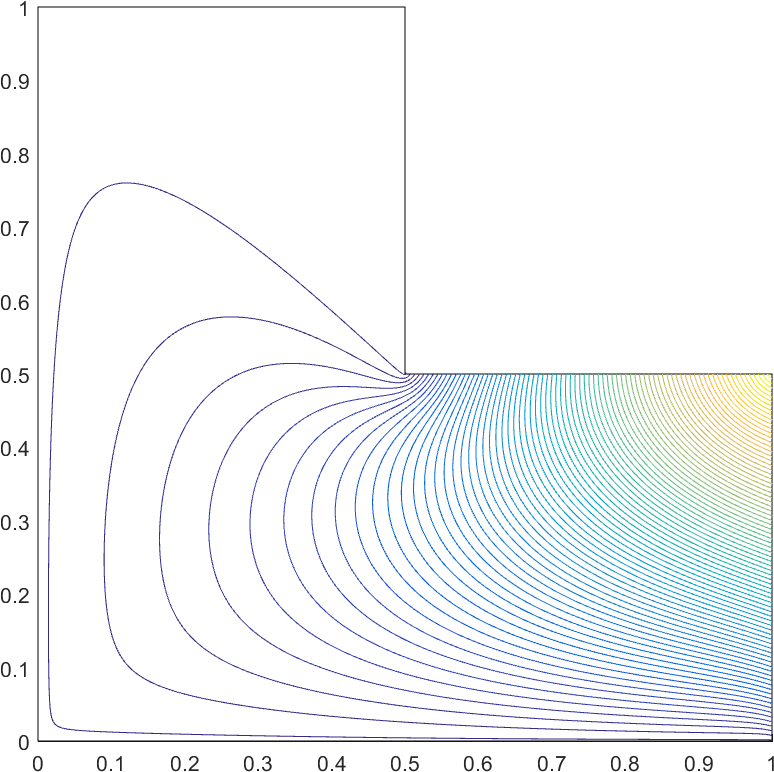
\includegraphics[width=\textwidth]{figures/sec_BF/L-domain_MV1_contour_b3.png}
		\caption{}
	\end{subfigure}
	\vfill
	\begin{subfigure}[b]{0.39\textwidth}
		\centering
		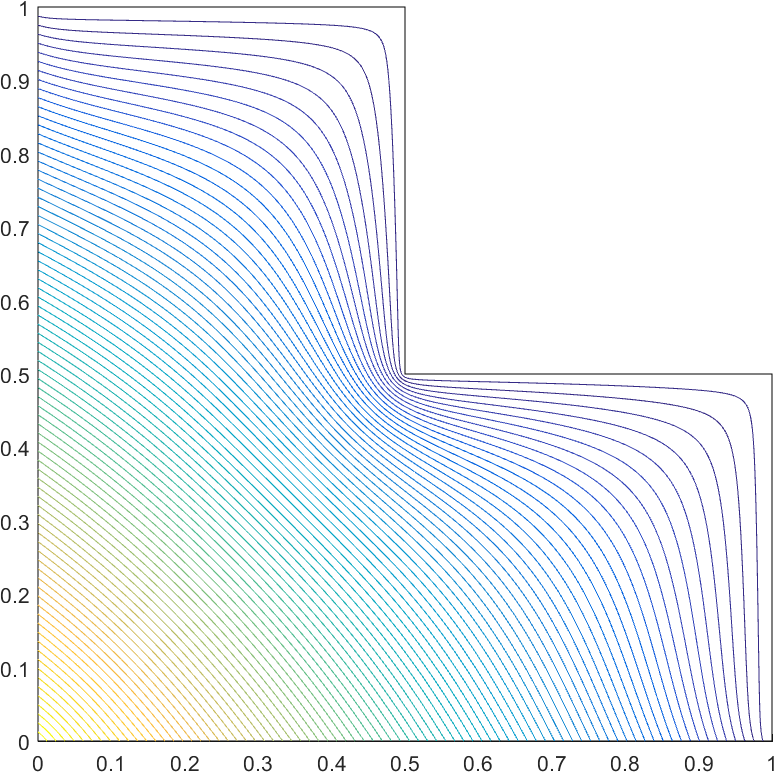
\includegraphics[width=\textwidth]{figures/sec_BF/L-domain_MV1_contour_b1.png}
		\caption{}
	\end{subfigure}
	\hspace{1.5cm}
	\begin{subfigure}[b]{0.39\textwidth}
		\centering
		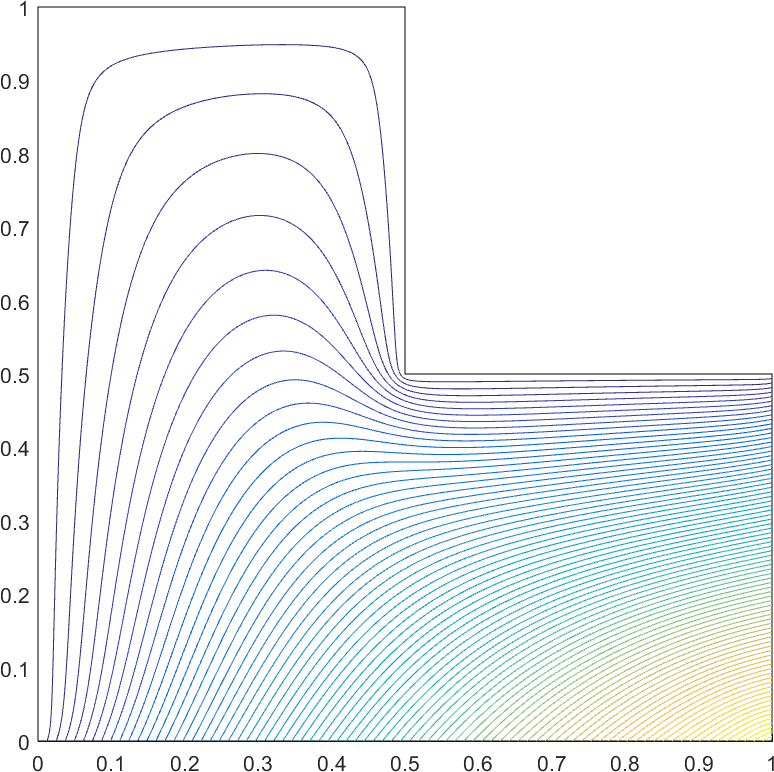
\includegraphics[width=\textwidth]{figures/sec_BF/L-domain_MV1_contour_b2.png}
		\caption{}
	\end{subfigure}
\caption{Contour plots of the linear mean value basis functions on the L-shaped domain for the vertices located at: (a) (0,1), (b) (1/2,1), (c) (1/2,1/2), (d) (1,1/2), (e) (0,0), and (f) (1,0).}
\end{figure}

%%%%%%%%%%%%%%%%%%%%%%%%%%%%%%%%%%%%%%%%%%%%%%%%%%%
%%%   SubSection - Maximum Entropy
\subsection{Maximum Entropy Basis Functions}
\label{sec::BF_2DLinear_ME}

The final linearly-complete 2D basis functions that we will analyze in this work are generated by use of the {\em maximum entropy coordinates} (ME) \cite{sukumar2004construction,arroyo2006local,hormann2008maximum}. 

\begin{equation}
\label{eq::BF_ME_BF}
b_{j}^{ME} (\vec{x}) = \frac{w_j (\vec{x}) }{\sum_i w_i (\vec{x})} .
\end{equation}

\noindent where the maximum entropy weight function for vertex $j$, $w_j$, has the following definition,

\begin{equation}
\label{eq::BF_ME_weights}
w_j (\vec{x})  = m_j(\vec{x}) \exp(-  \kappa \cdot (\vec{x}_j - \vec{x})),
\end{equation}

\noindent where $\kappa$ is a vector value of dimension $d$ that will be explained shortly. In Eq. (\ref{eq::BF_ME_weights}), $m_j$ is called the prior distribution and is a key component of Bayesian inference \cite{kullback1951information,jaynes1963information}. In the context of Eq. (\ref{eq::BF_ME_weights}), the prior distribution $m_j$ can be viewed as a weight function associated with vertex $j$. This means that there is variability that one can employ for these weight functions. These weight functions can then be tailored depending on the application and the numerical scheme employed. 

\begin{equation}
\label{eq::BF_ME_prior_funcs}
 m_j(\vec{x}) = \frac{\pi_j (\vec{x}) }{\sum_{k} \pi_k (\vec{x})}
\end{equation}

\noindent where

\begin{equation}
\label{eq::BF_ME_prior_products}
\pi_j (\vec{x}) = \prod\displaylimits_{i \neq j-1, j} \rho_j (\vec{x})
\end{equation}

\noindent where

\begin{equation}
\label{eq::BF_ME_face_funcs}
\rho_j (\vec{x}) = || \vec{x} - \vec{x}_j || + || \vec{x} - \vec{x}_{j+1} || - || \vec{x}_{j+1} - \vec{x}_j ||
\end{equation}

\begin{figure}
\label{fig::2D_MAXENT1_unit_square_basis_functions}
\centering
	\begin{subfigure}[b]{0.39\textwidth}
		\centering
		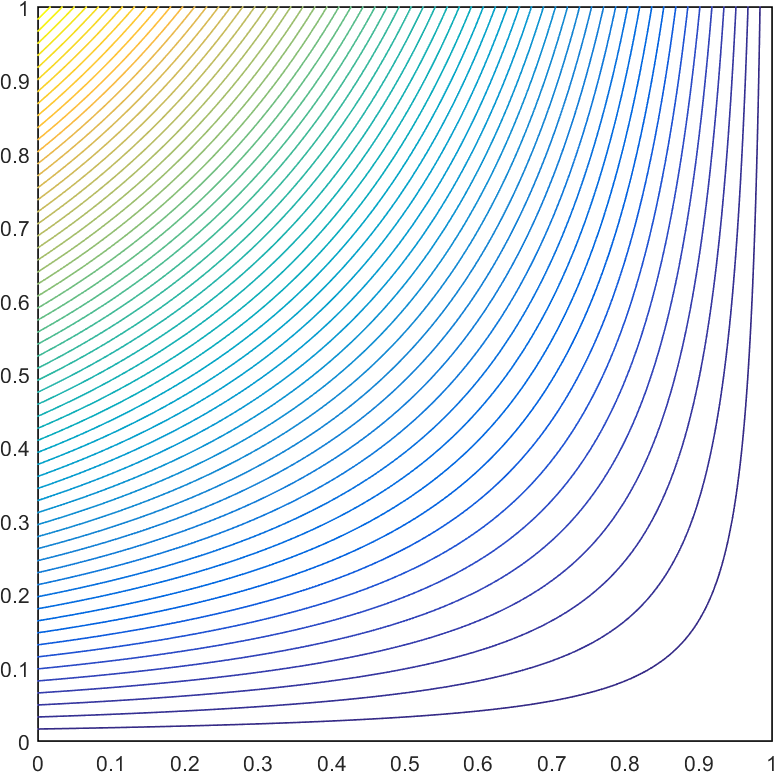
\includegraphics[width=\textwidth]{figures/sec_BF/square_MAXENT1_contour_b4.png}
		\caption{}
	\end{subfigure}
	\hspace{1.5cm}
	\begin{subfigure}[b]{0.39\textwidth}
		\centering
		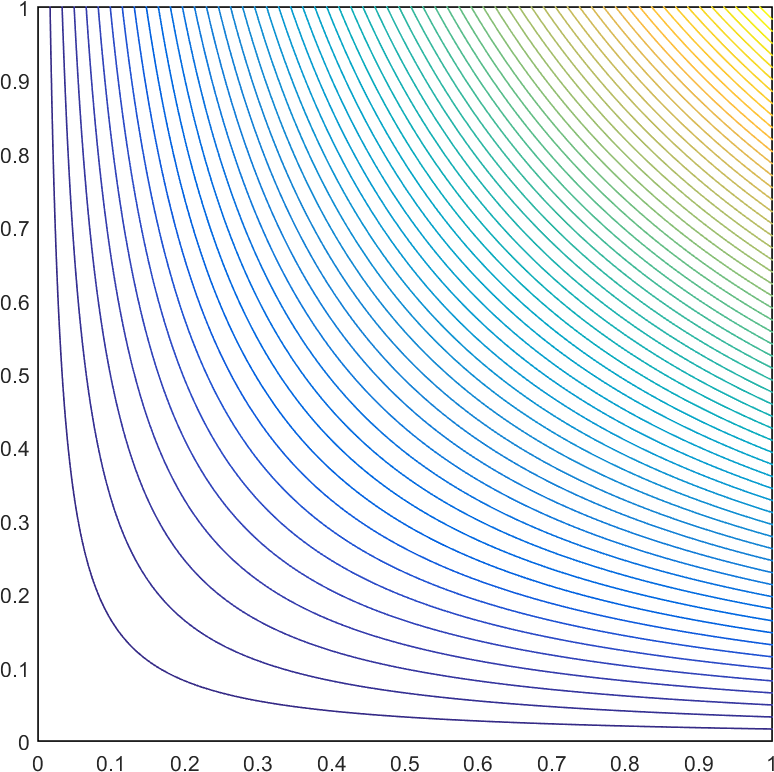
\includegraphics[width=\textwidth]{figures/sec_BF/square_MAXENT1_contour_b3.png}
		\caption{}
	\end{subfigure}
	\vfill
	\begin{subfigure}[b]{0.39\textwidth}
		\centering
		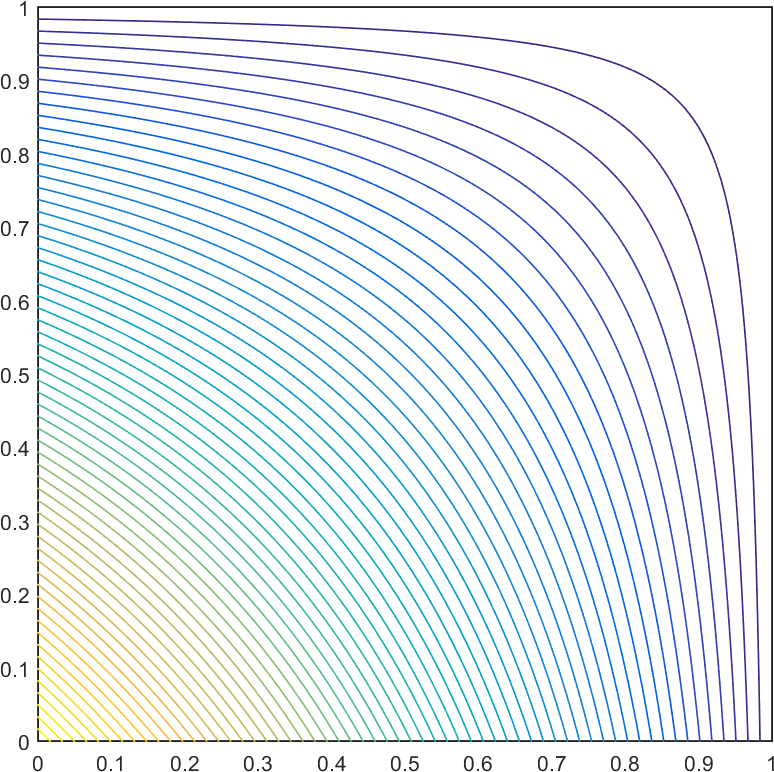
\includegraphics[width=\textwidth]{figures/sec_BF/square_MAXENT1_contour_b1.png}
		\caption{}
	\end{subfigure}
	\hspace{1.5cm}
	\begin{subfigure}[b]{0.39\textwidth}
		\centering
		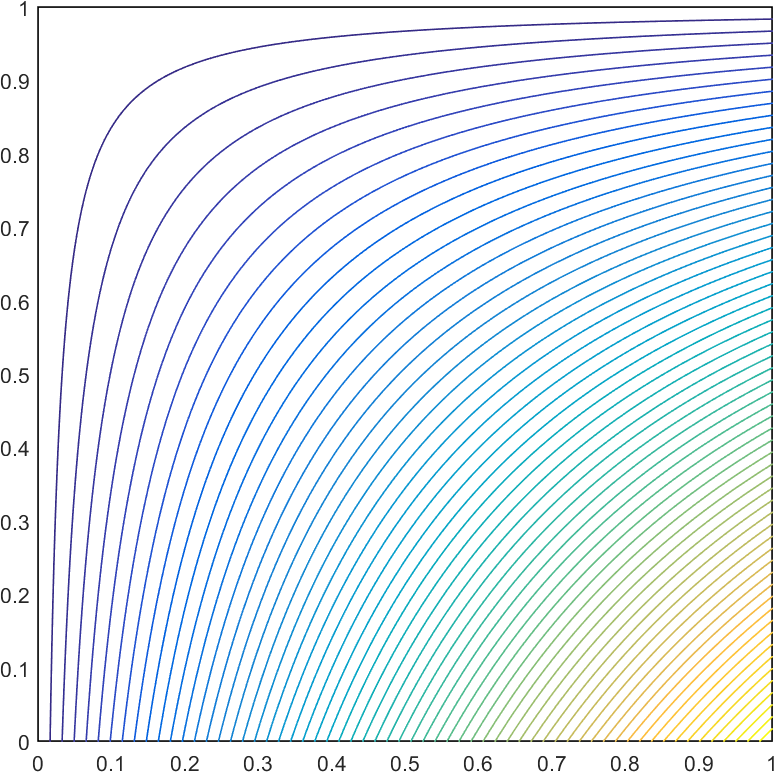
\includegraphics[width=\textwidth]{figures/sec_BF/square_MAXENT1_contour_b2.png}
		\caption{}
	\end{subfigure}
\caption{Contour plots of the linear maximum entropy basis functions on the unit square for the vertices located at: (a) (0,1), (b) (1,1), (c) (0,0), and (d) (1,0).}
\end{figure}

\begin{figure}
\label{fig::2D_MAXENT1_deg_square_basis_functions}
\centering
	\begin{subfigure}[b]{0.39\textwidth}
		\centering
		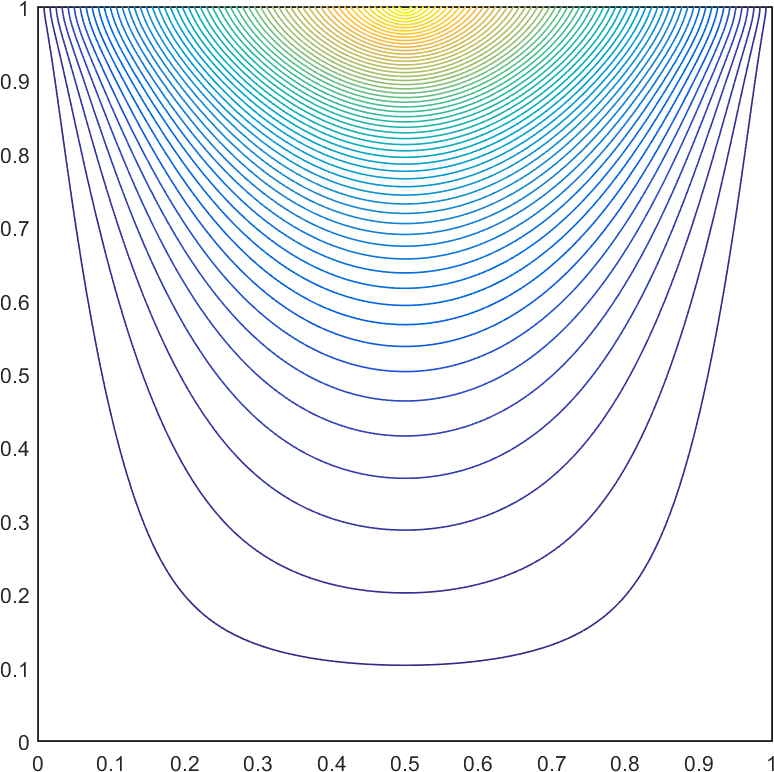
\includegraphics[width=\textwidth]{figures/sec_BF/deg_square_MAXENT1_contour_b4.png}
		\caption{}
	\end{subfigure}
	\vfill
	\begin{subfigure}[b]{0.39\textwidth}
		\centering
		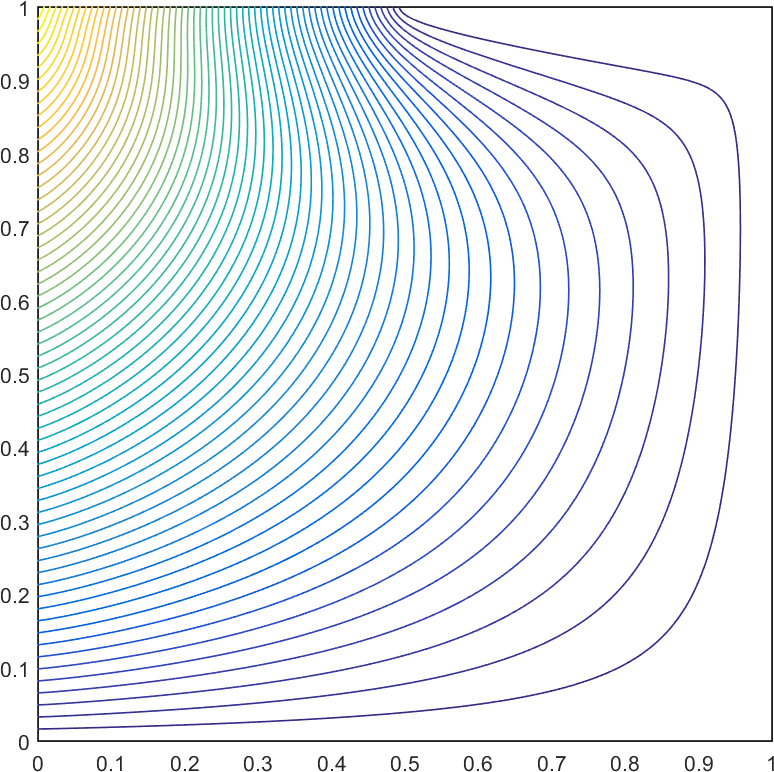
\includegraphics[width=\textwidth]{figures/sec_BF/deg_square_MAXENT1_contour_b5.png}
		\caption{}
	\end{subfigure}
	\hspace{1.5cm}
	\begin{subfigure}[b]{0.39\textwidth}
		\centering
		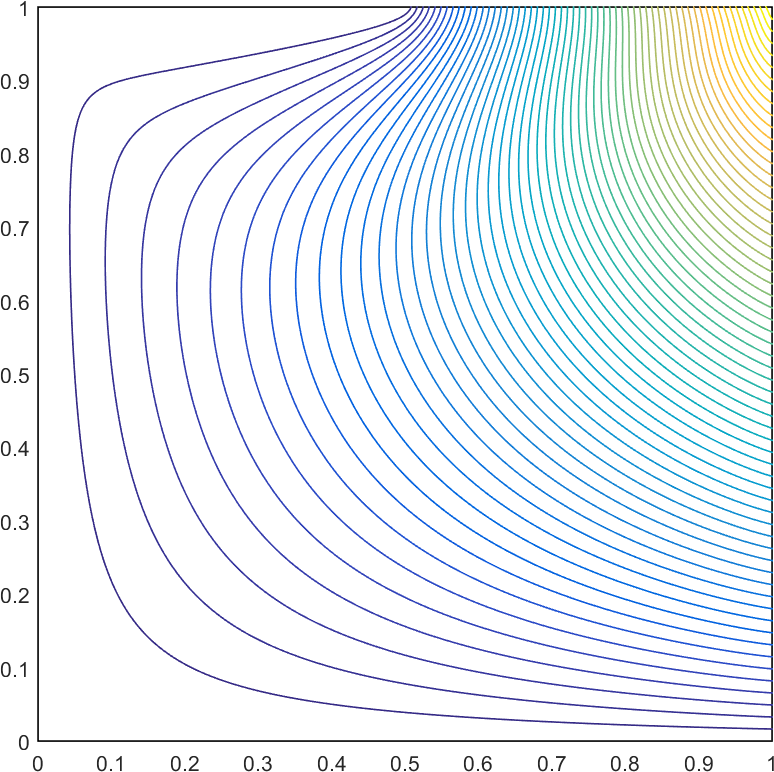
\includegraphics[width=\textwidth]{figures/sec_BF/deg_square_MAXENT1_contour_b3.png}
		\caption{}
	\end{subfigure}
	\vfill
	\begin{subfigure}[b]{0.39\textwidth}
		\centering
		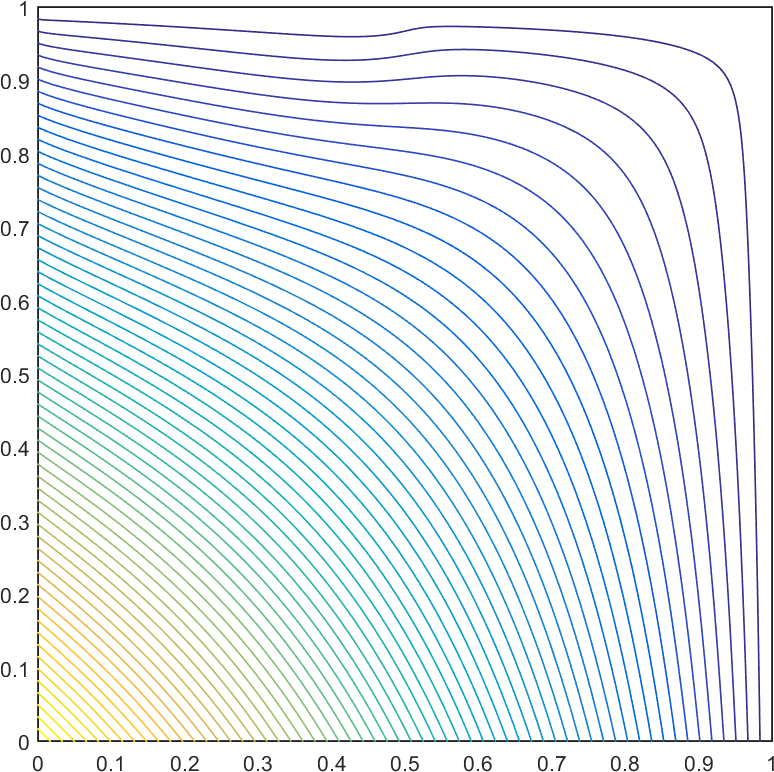
\includegraphics[width=\textwidth]{figures/sec_BF/deg_square_MAXENT1_contour_b1.png}
		\caption{}
	\end{subfigure}
	\hspace{1.5cm}
	\begin{subfigure}[b]{0.39\textwidth}
		\centering
		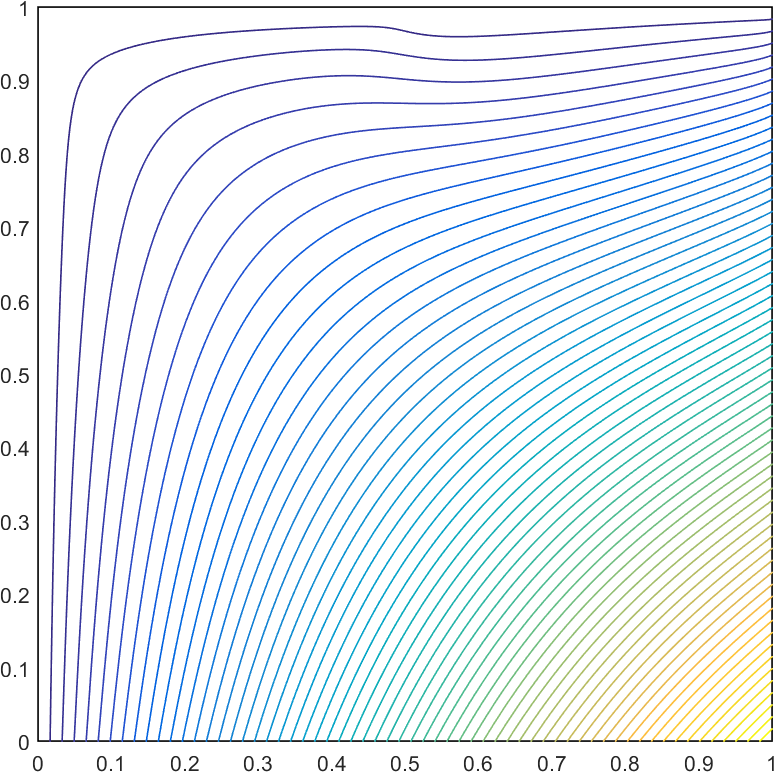
\includegraphics[width=\textwidth]{figures/sec_BF/deg_square_MAXENT1_contour_b2.png}
		\caption{}
	\end{subfigure}
\caption{Contour plots of the linear maximum entropy basis functions on the degnerate pentagon for the vertices located at: (a) (1/2,1), (b) (0,1), (c) (1,1), (d) (0,0), and (e) (1,0).}
\end{figure}

\begin{figure}
\label{fig::2D_MAXENT1_Ldom_basis_functions}
\centering
	\begin{subfigure}[b]{0.39\textwidth}
		\centering
		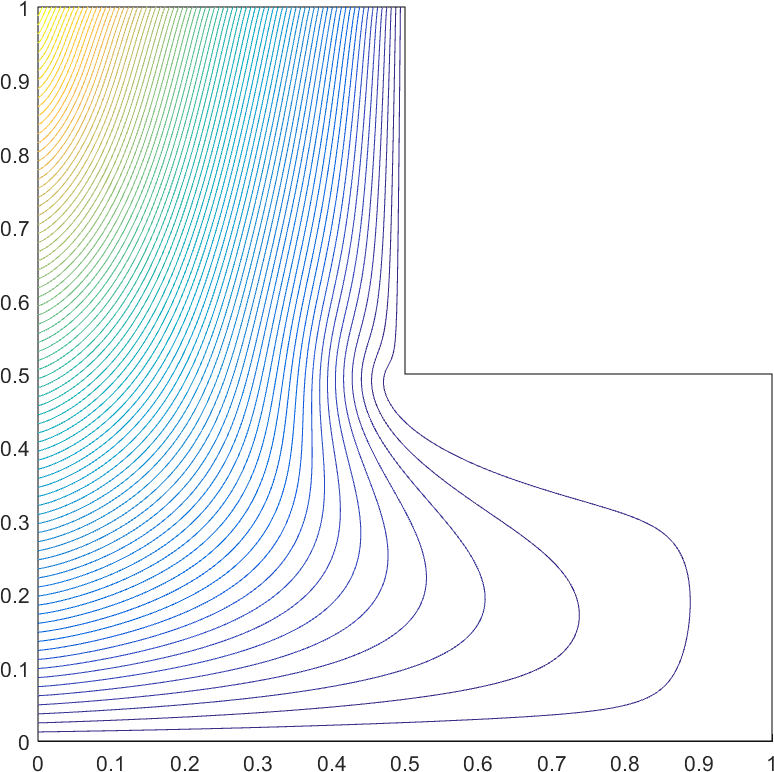
\includegraphics[width=\textwidth]{figures/sec_BF/L-domain_MAXENT1_contour_b6.png}
		\caption{}
	\end{subfigure}
	\hspace{1.5cm}
	\begin{subfigure}[b]{0.39\textwidth}
		\centering
		\includegraphics[width=\textwidth]{figures/sec_BF/L-domain_MAXENT1_contour_b5.png}
		\caption{}
	\end{subfigure}
	\vfill
	\begin{subfigure}[b]{0.39\textwidth}
		\centering
		\includegraphics[width=\textwidth]{figures/sec_BF/L-domain_MAXENT1_contour_b4.png}
		\caption{}
	\end{subfigure}
	\hspace{1.5cm}
	\begin{subfigure}[b]{0.39\textwidth}
		\centering
		\includegraphics[width=\textwidth]{figures/sec_BF/L-domain_MAXENT1_contour_b3.png}
		\caption{}
	\end{subfigure}
	\vfill
	\begin{subfigure}[b]{0.39\textwidth}
		\centering
		\includegraphics[width=\textwidth]{figures/sec_BF/L-domain_MAXENT1_contour_b1.png}
		\caption{}
	\end{subfigure}
	\hspace{1.5cm}
	\begin{subfigure}[b]{0.39\textwidth}
		\centering
		\includegraphics[width=\textwidth]{figures/sec_BF/L-domain_MAXENT1_contour_b2.png}
		\caption{}
	\end{subfigure}
\caption{Contour plots of the linear maximum entropy basis functions on the L-shaped domain for the vertices located at: (a) (0,1), (b) (1/2,1), (c) (1/2,1/2), (d) (1,1/2), (e) (0,0), and (f) (1,0).}
\end{figure}

%%%%%%%%%%%%%%%%%%%%%%%%%%%%%%%%%%%%%%%%%%%%%%%%%%%
%%%   SubSection - 2D linear summary
\subsection{Summary of 2D Linear Basis Functions on Polygons}
\label{sec::BF_2DLinear_Summary}

\begin{table}
\caption[Summary of the 2D polygonal basis functions]{Summary of the 2D coordinate systems used on polygons. }
\begin{tabular}{|c|c|c|c|c|}
\hline
Basis Function & Dimension & Polytope Types & Integration & Direct/Iterative \\
\hline \hline
Wachspress	&2D/3D&	Convex&	Numerical	&Direct\\ \hline
PWL&	1D/2D/3D&	Convex/Concave&	Analytical	&Direct\\ \hline
Mean Value&	2D&	Convex/Concave&	Numerical	&Direct\\ \hline
Max Entropy&	1D/2D/3D	&Convex/Concave&	Numerical&	Iterative\\ \hline
\end{tabular}
\end{table}

\begin{figure}
\label{fig::2D_Linear_Summary_unit_square_basis_functions}
\centering
	\begin{subfigure}[b]{0.39\textwidth}
		\centering
		\includegraphics[width=\textwidth]{figures/sec_BF/square_WACHSPRESS1_contour_b4.png}
		\caption{}
	\end{subfigure}
	\hspace{1.5cm}
	\begin{subfigure}[b]{0.39\textwidth}
		\centering
		\includegraphics[width=\textwidth]{figures/sec_BF/square_PWLD1_contour_b4.png}
		\caption{}
	\end{subfigure}
	\vfill
	\begin{subfigure}[b]{0.39\textwidth}
		\centering
		\includegraphics[width=\textwidth]{figures/sec_BF/square_MV1_contour_b4.png}
		\caption{}
	\end{subfigure}
	\hspace{1.5cm}
	\begin{subfigure}[b]{0.39\textwidth}
		\centering
		\includegraphics[width=\textwidth]{figures/sec_BF/square_MAXENT1_contour_b4.png}
		\caption{}
	\end{subfigure}
\caption[Contour plots of the linear basis functions on the unit square.]{Contour plots of the different linear basis function on the unit square located at vertex (0,1): (a) Wachspress, (b) PWL, (c) mean value, and (d) maximum entropy.}
\end{figure}

\begin{figure}
\label{fig::2D_Summary_deg_square_basis_functions}
\centering
	\begin{subfigure}[b]{0.39\textwidth}
		\centering
		\includegraphics[width=\textwidth]{figures/sec_BF/deg_square_WACHSPRESS1_contour_b5.png}
		\caption{}
	\end{subfigure}
	\hspace{1.5cm}
	\begin{subfigure}[b]{0.39\textwidth}
		\centering
		\includegraphics[width=\textwidth]{figures/sec_BF/deg_square_PWLD1_contour_b5.png}
		\caption{}
	\end{subfigure}
	\vfill
	\begin{subfigure}[b]{0.39\textwidth}
		\centering
		\includegraphics[width=\textwidth]{figures/sec_BF/deg_square_MV1_contour_b5.png}
		\caption{}
	\end{subfigure}
	\hspace{1.5cm}
	\begin{subfigure}[b]{0.39\textwidth}
		\centering
		\includegraphics[width=\textwidth]{figures/sec_BF/deg_square_MAXENT1_contour_b5.png}
		\caption{}
	\end{subfigure}
\caption[Contour plots of the linear basis functions on the degenerate pentagon.]{Contour plots of the different linear basis function on the degenerate pentagon located at vertex (0,1): (a) Wachspress, (b) PWL, (c) mean value, and (d) maximum entropy.}
\end{figure}

%%%%%%%%%%%%%%%%%%%%%%%%%%%%%%%%%%%%%%%%%%%%%%%%%%%
%%%   Section - Quadratic Basis Functions
\section{Quadratic Serendipity Basis Functions on 2D Polygons}
\label{sec::BF_2DQuadratic}

for the constant constraint,

\begin{equation}
\label{eq::BF_quad_interp_req_constant}
\sum_{i=1}^{2 N_K}  b_i (\vec{x})  = 1 ,
\end{equation}

\noindent for the linear constraint,

\begin{equation}
\label{eq::BF_quad_interp_req_linear}
\sum_{i=1}^{2 N_K}  b_i (\vec{x}) \left( \vec{x}_i -\vec{x}  \right)= \vec{0} ,
\end{equation}

\noindent and for the quadratic constraint,

\begin{equation}
\label{eq::BF_quad_interp_req_quadratic}
\sum_{i=1}^{2 N_K}  b_i (\vec{x}) \left[  \left( \vec{x}_i -\vec{x}  \right) \otimes \left( \vec{x}_i -\vec{x}  \right) - \vec{d}_i   \right] =  \vec{0} .
\end{equation}

\noindent In Eq. (\ref{eq::BF_quad_interp_req_quadratic}), the nodal coefficients, $\vec{d}_i$, have the interpretation of being the nodal gap functions \cite{rosolen2013second}. This ensures the reproduction of our second-order convex approximation scheme. These nodal gap functions have the form for the vertex functions of,

\begin{equation}
\label{eq::BF_quad_nodal gaps_verts}
\vec{d}_i = \vec{0}, \qquad i \in (1,N_K) ,
\end{equation}

\noindent and the form on the face midpoints of,

\begin{equation}
\label{eq::BF_quad_nodal gaps_edges}
\vec{d}_{a+N_K} = \frac{ \left( \vec{x}_{a+1} -\vec{x}_a  \right) \otimes \left( \vec{x}_{a+1} -\vec{x}_a   \right) }{4}, \qquad   1 \leq a \leq N_K.
\end{equation}

\begin{equation}
\label{eq::BF_quad_interp_req_vector}
\sum_{i=1}^{N_K}  b_i (\vec{x}) \vec{c}_{i,2}(\vec{x}) = \vec{q}_2 ,
\end{equation}


\begin{equation}
\label{eq::BF_quad_MP_inverse}
B^* = B^T (B B^T)^{-1}
\end{equation}


%%%%%%%%%%%%%%%%%%%%%%%%%%%%%%%%%%%%%%%%%%%%%%%%%%%
%%%   SubSection -Analytical PWQ
\subsection{Analytical Form of the Quadratic Serendipity Extension of the PWL Functions}
\label{sec::BF_2DQuadratic_PWQ}



%%%%%%%%%%%%%%%%%%%%%%%%%%%%%%%%%%%%%%%%%%%%%%%%%%%
%%%   SubSection - 2D quadratic summary
\subsection{Summary of 2D Quadratic Serendipity Basis Functions on Polygons}
\label{sec::BF_2DQuadratic_Summary}

\begin{figure}
\label{fig::2D_Quadratic_Summary_unit_square_basis_functions_BF4}
\centering
	\begin{subfigure}[b]{0.39\textwidth}
		\centering
		\includegraphics[width=\textwidth]{figures/sec_BF/square_WACHSPRESS2_contour_b4.png}
		\caption{}
	\end{subfigure}
	\hspace{1.5cm}
	\begin{subfigure}[b]{0.39\textwidth}
		\centering
		\includegraphics[width=\textwidth]{figures/sec_BF/square_PWLD2_contour_b4.png}
		\caption{}
	\end{subfigure}
	\vfill
	\begin{subfigure}[b]{0.39\textwidth}
		\centering
		\includegraphics[width=\textwidth]{figures/sec_BF/square_MV2_contour_b4.png}
		\caption{}
	\end{subfigure}
	\hspace{1.5cm}
	\begin{subfigure}[b]{0.39\textwidth}
		\centering
		\includegraphics[width=\textwidth]{figures/sec_BF/square_MAXENT2_contour_b4.png}
		\caption{}
	\end{subfigure}
\caption[Contour plots of the quadratic basis functions on the unit square.]{Contour plots of the different quadratic serendipity basis function on the unit square located at vertex (0,1): (a) Wachspress, (b) PWL, (c) mean value, and (d) maximum entropy.}
\end{figure}

\begin{figure}
\label{fig::2D_Quadratic_Summary_unit_square_basis_functions_BF8}
\centering
	\begin{subfigure}[b]{0.39\textwidth}
		\centering
		\includegraphics[width=\textwidth]{figures/sec_BF/square_WACHSPRESS2_contour_b8.png}
		\caption{}
	\end{subfigure}
	\hspace{1.5cm}
	\begin{subfigure}[b]{0.39\textwidth}
		\centering
		\includegraphics[width=\textwidth]{figures/sec_BF/square_PWLD2_contour_b8.png}
		\caption{}
	\end{subfigure}
	\vfill
	\begin{subfigure}[b]{0.39\textwidth}
		\centering
		\includegraphics[width=\textwidth]{figures/sec_BF/square_MV2_contour_b8.png}
		\caption{}
	\end{subfigure}
	\hspace{1.5cm}
	\begin{subfigure}[b]{0.39\textwidth}
		\centering
		\includegraphics[width=\textwidth]{figures/sec_BF/square_MAXENT2_contour_b8.png}
		\caption{}
	\end{subfigure}
\caption[Contour plots of the quadratic basis functions on the unit square.]{Contour plots of the different quadratic serendipity basis function on the unit square at a mid-face node located at (0,1/2): (a) Wachspress, (b) PWL, (c) mean value, and (d) maximum entropy.}
\end{figure}

%%%%%%%%%%%%%%%%%%%%%%%%%%%%%%%%%%%%%%%%%%%%%%%%%%%
%%%   Section - Integrating 2D Polygons
\section{Integrating the Arbitrary 2D Polygonal Elements}
\label{sec::BF_2DIntegration}


%%%%%%%%%%%%%%%%%%%%%%%%%%%%%%%%%%%%%%%%%%%%%%%%%%%
%%%   Section - 3D
\section{Linear Basis Functions on 3D Polyhedra}
\label{sec::BF_3DLinear}



%%%%%%%%%%%%%%%%%%%%%%%%%%%%%%%%%%%%%%%%%%%%%%%%%%%
%%%   SubSection - 3D Lin/TriL
\subsection{3D Linear and TriLinear Basis Functions}
\label{sec::BF_3DLinear_TriL}

\begin{figure}
\centering
	\begin{subfigure}[b]{0.45\textwidth}
		\centering
		\label{subfig::unit_square}
		\includegraphics[width=\textwidth]{figures/sec_BF/unit_square_linear.eps}
		\caption{}
	\end{subfigure}
	\hfill
	\begin{subfigure}[b]{0.45\textwidth}
		\centering
		\label{subfig::unit_cube}
		\includegraphics[width=\textwidth]{figures/sec_BF/unit_cube_linear.eps}
		\caption{}
	\end{subfigure}
\caption{Vertex structure for the (a) unit square and (b) unit cube.}
\label{fig::BF_3D_unit_tet_cube}
\end{figure}

\begin{equation}
\label{eq::3D_lin_basis_functions}
\begin{aligned}
	b_1(r,s) & = 1-r-s-t \\
	b_2(r,s) & = r \\
	b_3(r,s) & = s \\
	b_4(r,s) & = t
\end{aligned}
\end{equation}

\noindent and

\begin{equation}
\label{eq::TriL_basis_functions}
\begin{aligned}
	b_1(r,s,t) & = (1-r)(1-s)(1-t) \\
	b_2(r,s,t) & = r(1-s)(1-t) \\
	b_3(r,s,t) & = rs(1-t) \\
	b_4(r,s,t) & = (1-r)s(1-t) \\
	b_5(r,s,t) & = (1-r)(1-s)t \\
	b_6(r,s,t) & = r(1-s)t \\
	b_7(r,s,t) & = rst \\
	b_8(r,s,t) & = (1-r)st \\
\end{aligned}
\end{equation}

%%%%%%%%%%%%%%%%%%%%%%%%%%%%%%%%%%%%%%%%%%%%%%%%%%%
%%%   SubSection - PWL
\subsection{3D Piecewise Linear (PWL) Basis Functions}
\label{sec::BF_3DLinear_PWL}

The 3D PWL basis functions share a similar form to the 2D PWL basis functions.

\begin{equation}
\label{eq::PWL_3D}
	b_j (x,y,z)  = t_j  (x,y,z) + \sum_{f=1}^{F_j} \beta_f^j  t_f (x,y,z) + \alpha_j^K t_c  (x,y,z)
\end{equation}

\noindent $t_j$ is the standard 3D linear function with unity at vertex $j$ that linearly decreases to zero to the cell center, the face center for each face that includes vertex $j$, and each vertex that shares an edge with vertex $j$. $t_c$ is the 3D cell ``tent" function which is unity at the cell center and linearly decreases to zero to each cell vertex and face center. $t_f$ is the face "tent" function which is unity at the face center and linearly decreases to zero at each vertex on that face and the cell center. $\beta_{f,j}$ is the weight parameter for face $f$ touching cell vertex $j$, and $F_j$ is the number of faces touching vertex $j$. Like the previous work defining the PWLD method \cite{bailey2008phd}, we also choose to assume the cell and face weighting parameters are

\begin{equation}
\alpha_{K,j} = \frac{1}{N_K} \qquad \text{and} \qquad \beta_{f,j} = \frac{1}{N_f},
\label{eq::PWL_weight_vals}
\end{equation}

\noindent respectively, where $N_K$ is the number of vertices in cell $K$ and $N_f$ is the number of vertices on face $f$, which leads to constant values of $\alpha$ and $\beta$ for each cell and face, respectively. This assumption of the cell weight function holds for both 2D and 3D.

%%%%%%%%%%%%%%%%%%%%%%%%%%%%%%%%%%%%%%%%%%%%%%%%%%%
%%%   Section - Results
\section{Numerical Results}
\label{sec::BF_Results}

Now that we have presented several linear polygonal finite element basis sets along with the methodology to convert them to quadratic serendipity-like basis, we present several numerical problems to demonstrate our methodology. First, we demonstrate that the presented basis sets can capture an exactly-linear transport solution in Section \ref{sec::BF_Results_Linear}. Next, we present some convergence properties of the basis sets using the method of manufactured solutions (MMS) in Section \ref{sec::BF_Results_MMS}. We then present a searchlight problem and observe how the basis sets react with adaptive mesh refinement (AMR) to mitigate numerical dispersion through a vacuum in Section \ref{sec::BF_Results_SL}.

%%%%%%%%%%%%%%%%%%%%%%%%%%%%%%%%%%%%%%%%%%%%%%%%%%%
%%%   SubSection - Linear Solutions = METHOD OF EXACT SOLUTIONS
\newpage
\subsection{Two-Dimensional Exactly-Linear Transport Solutions}
\label{sec::BF_Results_Linear}

We present our first numerical example by demonstrating that the linear and quadratic polygonal finite element basis functions capture an exactly-linear solution space. We will show this by the method of exact solutions (MES). Since the coordinate interpolation of the basis functions for the linear basis functions requires exact linear interpolation (Eq. (\ref{eq::BF_linear_interp_affine})), then an exactly-linear solution space can be captured, even on highly distorted polygonal meshes. This also applies to the quadratic serendipity space since it is formed by the product-wise pairings of the linear basis functions. We build our exact solution by investigating the 2D, 1 energy group transport problem with no scattering and an angle-dependent distributed source,

\begin{equation}
\label{eq::BF_Results_Linear_angflux}
\mu \frac{\partial \Psi}{\partial x} + \eta \frac{\partial \Psi}{\partial y} + \sigma_t \Psi = Q(x,y, \mu, \eta), 
\end{equation}

\noindent where the streaming term was separated into the corresponding two-dimensional terms. We chose to drop the scattering term for this example so that the error arising from iteratively converging our solution would have no impact.

We then define an angular flux solution that is linear in both space and angle along with the corresponding 0th moment scalar flux ($\Phi_{0,0} \rightarrow \Phi$) solution:

\begin{equation}
\label{eq::BF_Results_Linear_fluxsols}
\begin{aligned}
\Psi (x,y,\mu,\eta) &= ax + by + c \mu + d\eta + e\\
\Phi (x,y) &= 2 \pi \left( ax + by  + e \right)
\end{aligned} .
\end{equation}

\noindent One can immediately notice that our 0th moment solution is not dependent on angle. We arrive at this solution by enforcing our 2D angular quadrature set to have the following properties:

\begin{equation}
\label{eq::BF_Results_Linear_quadrules}
\sum_{q} w_q = 2 \pi \qquad \text{and} \qquad \sum_{q} w_q  \left[
	\begin{array}{c}
		\mu_q \\
		\eta_q
	\end{array} \right] = \left[
	\begin{array}{c}
		0 \\
		0
	\end{array} \right] .
\end{equation}

\noindent The sum of the quadrature weights is handled by simply renormalizing those that are generated in Section \ref{sec::Sn_Angle} to $2 \pi$.

Our boundary conditions for all inflow boundaries are then uniquely determined by the angular flux solution of Eq. (\ref{eq::BF_Results_Linear_fluxsols}). Inserting the angular flux solution of Eq. (\ref{eq::BF_Results_Linear_fluxsols}) into Eq. (\ref{eq::BF_Results_Linear_angflux}), we obtain the distributed source that will produce our exactly-linear solution space:

\begin{equation}
\label{eq::BF_Results_Linear_src}
Q(x,y,\mu,\eta) = a \mu + b \eta + \sigma_t \left(  c \mu + d \eta \right) + \sigma_t \left( ax +by + e   \right).
\end{equation}

\noindent It is noted that the angular dependence of the source can be removed (which can ease the code development burden) if one sets

\begin{equation}
\label{eq::BF_Results_Linear_removeterms}
\begin{aligned}
	a &= - c \, \sigma_t, \\
	b &= - d \, \sigma_t.
\end{aligned}
\end{equation}

For this example, we test the various 2D polygonal finite element basis functions on six different mesh types. These mesh types include triangular, quadrilateral, and polygonal meshes:

\begin{enumerate}
	\item Orthogonal cartesian mesh formed by the intersection of 11 equally-spaced vertices in both the $x$ and $y$ dimensions. This forms a 10x10 array of quadrilateral mesh cells.
	\item Ordered-triangular mesh formed by the bisection of the previous orthogonal cartesian mesh (forming 200 triangles all of the same size/shape).
	\item Quadrilateral shestakov grid formed by the randomization of vertices based on a skewness parameter \cite{shestakov1988solution,shestakov1990test}. With a certain range of this skewness parameter, highly distorted meshes can be generated.
	\item Sinusoidal polygonal grid that is generated by the transformation of a uniform orthogonal grid based on a sinusoid functional. The transformed vertices are then converted into a polygonal grid by computing a bounded Voronoi diagram.
	\item Kershaw's quadrilateral z-mesh \cite{kershaw1981differencing}. This mesh is formed by taking an orthogonal quadrilateral grid and displacing certain interior vertices only in the $y$ dimension.
	\item A polygonal variant of the quadrilateral z-mesh. The polygonal grid is formed in a similar manner to the sinusoidal polygonal mesh with a Voronoi diagram.
\end{enumerate}

\noindent We also wish that both the angular flux solution as well as the 0th moment solution are strictly positive everywhere. Therefore, we set the function parameters in Eq. (\ref{eq::BF_Results_Linear_fluxsols}) to $\sigma_t = a = c = d = e = 1.0$ and $b = 1.5$. We gave the solution the $40 \%$ tilt in space ($a \neq b$) so that it would not align with the triangular mesh. Using an S8 LS quadrature set, we ran all combinations of the polygonal basis functions and the mesh types. The linear solutions for the Wachspress, PWL, mean value, linear maximum entropy, and quadratic serendipity maximum entropy basis functions are presented in Figures \ref{fig::BF_Results_Linear_wach_sol}, \ref{fig::BF_Results_Linear_pwld_sol}, \ref{fig::BF_Results_Linear_mv_sol}, \ref{fig::BF_Results_Linear_me1_sol}, and \ref{fig::BF_Results_Linear_me2_sol}, respectively. We can see that for all the polygonal basis functions, an exact linear solution is captured as shown by the unbroken nature of the contour lines. This even holds on the highly distorted quadrilateral shestakov mesh.

%%%%%%%%%%%%%%%%%
% Begin Linear Solution figures
\begin{figure}
\centering
	\begin{subfigure}[b]{0.45\textwidth}
		\centering
		\label{subfig::cart_wach_lin_sol}
		\includegraphics[width=\textwidth]{figures/sec_BF/cart_WACHSPRESS_k1.eps}
		\caption{}
	\end{subfigure}
	\hfill
	\begin{subfigure}[b]{0.45\textwidth}
		\centering
		\label{subfig::tri_wach_lin_sol}
		\includegraphics[width=\textwidth]{figures/sec_BF/tri_WACHSPRESS_k1.eps}
		\caption{}
	\end{subfigure}
	\vfill
	\begin{subfigure}[b]{0.45\textwidth}
		\centering
		\label{subfig::shes_quad_wach_lin_sol}
		\includegraphics[width=\textwidth]{figures/sec_BF/shes_quad_WACHSPRESS_k1.eps}
		\caption{}
	\end{subfigure}
	\hfill
	\begin{subfigure}[b]{0.45\textwidth}
		\centering
		\label{subfig::smooth_poly_wach_lin_sol}
		\includegraphics[width=\textwidth]{figures/sec_BF/smooth_poly_WACHSPRESS_k1.eps}
		\caption{}
	\end{subfigure}
	\vfill
	\begin{subfigure}[b]{0.45\textwidth}
		\centering
		\label{subfig::z_quad_wach_lin_sol}
		\includegraphics[width=\textwidth]{figures/sec_BF/z_quad_WACHSPRESS_k1.eps}
		\caption{}
	\end{subfigure}
	\hfill
	\begin{subfigure}[b]{0.45\textwidth}
		\centering
		\label{subfig::z_poly_wach_lin_sol}
		\includegraphics[width=\textwidth]{figures/sec_BF/z_poly_WACHSPRESS_k1.eps}
		\caption{}
	\end{subfigure}
\caption{Contour plots of the exactly-linear solution with the Wachspress basis functions on (a) cartesian mesh, (b) ordered-triangular mesh, (c) quadrilateral shestakov mesh, (d) sinusoidal polygonal mesh, (e) quadrilateral z-mesh, and (f) polygonal z-mesh.}
\label{fig::BF_Results_Linear_wach_sol}
\end{figure}
% Begin false
\iffalse
\begin{figure}
\centering
	\begin{subfigure}[b]{0.45\textwidth}
		\centering
		\label{subfig::cart_pwld_lin_sol}
		\includegraphics[width=\textwidth]{figures/sec_BF/cart_PWLD_k1.eps}
		\caption{}
	\end{subfigure}
	\hfill
	\begin{subfigure}[b]{0.45\textwidth}
		\centering
		\label{subfig::tri_pwld_lin_sol}
		\includegraphics[width=\textwidth]{figures/sec_BF/tri_PWLD_k1.eps}
		\caption{}
	\end{subfigure}
	\vfill
	\begin{subfigure}[b]{0.45\textwidth}
		\centering
		\label{subfig::shes_quad_pwld_lin_sol}
		\includegraphics[width=\textwidth]{figures/sec_BF/shes_quad_PWLD_k1.eps}
		\caption{}
	\end{subfigure}
	\hfill
	\begin{subfigure}[b]{0.45\textwidth}
		\centering
		\label{subfig::smooth_poly_pwld_lin_sol}
		\includegraphics[width=\textwidth]{figures/sec_BF/smooth_poly_PWLD_k1.eps}
		\caption{}
	\end{subfigure}
	\vfill
	\begin{subfigure}[b]{0.45\textwidth}
		\centering
		\label{subfig::z_quad_pwld_lin_sol}
		\includegraphics[width=\textwidth]{figures/sec_BF/z_quad_PWLD_k1.eps}
		\caption{}
	\end{subfigure}
	\hfill
	\begin{subfigure}[b]{0.45\textwidth}
		\centering
		\label{subfig::z_poly_pwld_lin_sol}
		\includegraphics[width=\textwidth]{figures/sec_BF/z_poly_PWLD_k1.eps}
		\caption{}
	\end{subfigure}
\caption{Contour plots of the exactly-linear solution with the PWL basis functions on (a) cartesian mesh, (b) ordered-triangular mesh, (c) quadrilateral shestakov mesh, (d) sinusoidal polygonal mesh, (e) quadrilateral z-mesh, and (f) polygonal z-mesh.}
\label{fig::BF_Results_Linear_pwld_sol}
\end{figure}

\begin{figure}
\centering
	\begin{subfigure}[b]{0.45\textwidth}
		\centering
		\label{subfig::cart_mv_lin_sol}
		\includegraphics[width=\textwidth]{figures/sec_BF/cart_MV_k1.eps}
		\caption{}
	\end{subfigure}
	\hfill
	\begin{subfigure}[b]{0.45\textwidth}
		\centering
		\label{subfig::tri_mv_lin_sol}
		\includegraphics[width=\textwidth]{figures/sec_BF/tri_MV_k1.eps}
		\caption{}
	\end{subfigure}
	\vfill
	\begin{subfigure}[b]{0.45\textwidth}
		\centering
		\label{subfig::shes_quad_mv_lin_sol}
		\includegraphics[width=\textwidth]{figures/sec_BF/shes_quad_MV_k1.eps}
		\caption{}
	\end{subfigure}
	\hfill
	\begin{subfigure}[b]{0.45\textwidth}
		\centering
		\label{subfig::smooth_poly_mv_lin_sol}
		\includegraphics[width=\textwidth]{figures/sec_BF/smooth_poly_MV_k1.eps}
		\caption{}
	\end{subfigure}
	\vfill
	\begin{subfigure}[b]{0.45\textwidth}
		\centering
		\label{subfig::z_quad_mv_lin_sol}
		\includegraphics[width=\textwidth]{figures/sec_BF/z_quad_MV_k1.eps}
		\caption{}
	\end{subfigure}
	\hfill
	\begin{subfigure}[b]{0.45\textwidth}
		\centering
		\label{subfig::z_poly_mv_lin_sol}
		\includegraphics[width=\textwidth]{figures/sec_BF/z_poly_MV_k1.eps}
		\caption{}
	\end{subfigure}
\caption{Contour plots of the exactly-linear solution with the mean value basis functions on (a) cartesian mesh, (b) ordered-triangular mesh, (c) quadrilateral shestakov mesh, (d) sinusoidal polygonal mesh, (e) quadrilateral z-mesh, and (f) polygonal z-mesh.}
\label{fig::BF_Results_Linear_mv_sol}
\end{figure}

\begin{figure}
\centering
	\begin{subfigure}[b]{0.45\textwidth}
		\centering
		\label{subfig::cart_me_k1_lin_sol}
		\includegraphics[width=\textwidth]{figures/sec_BF/cart_MAXENT_k1.eps}
		\caption{}
	\end{subfigure}
	\hfill
	\begin{subfigure}[b]{0.45\textwidth}
		\centering
		\label{subfig::tri_me_k1_lin_sol}
		\includegraphics[width=\textwidth]{figures/sec_BF/tri_MAXENT_k1.eps}
		\caption{}
	\end{subfigure}
	\vfill
	\begin{subfigure}[b]{0.45\textwidth}
		\centering
		\label{subfig::shes_quad_me_k1_lin_sol}
		\includegraphics[width=\textwidth]{figures/sec_BF/shes_quad_MAXENT_k1.eps}
		\caption{}
	\end{subfigure}
	\hfill
	\begin{subfigure}[b]{0.45\textwidth}
		\centering
		\label{subfig::smooth_poly_me_k1_lin_sol}
		\includegraphics[width=\textwidth]{figures/sec_BF/smooth_poly_MAXENT_k1.eps}
		\caption{}
	\end{subfigure}
	\vfill
	\begin{subfigure}[b]{0.45\textwidth}
		\centering
		\label{subfig::z_quad_me_k1_lin_sol}
		\includegraphics[width=\textwidth]{figures/sec_BF/z_quad_MAXENT_k1.eps}
		\caption{}
	\end{subfigure}
	\hfill
	\begin{subfigure}[b]{0.45\textwidth}
		\centering
		\label{subfig::z_poly_me_k1_lin_sol}
		\includegraphics[width=\textwidth]{figures/sec_BF/z_poly_MAXENT_k1.eps}
		\caption{}
	\end{subfigure}
\caption{Contour plots of the exactly-linear solution with the linear maximum entropy basis functions on (a) cartesian mesh, (b) ordered-triangular mesh, (c) quadrilateral shestakov mesh, (d) sinusoidal polygonal mesh, (e) quadrilateral z-mesh, and (f) polygonal z-mesh.}
\label{fig::BF_Results_Linear_me1_sol}
\end{figure}

\begin{figure}
\centering
	\begin{subfigure}[b]{0.45\textwidth}
		\centering
		\label{subfig::cart_me_k2_lin_sol}
		\includegraphics[width=\textwidth]{figures/sec_BF/cart_MAXENT_k2.eps}
		\caption{}
	\end{subfigure}
	\hfill
	\begin{subfigure}[b]{0.45\textwidth}
		\centering
		\label{subfig::tri_me_k2_lin_sol}
		\includegraphics[width=\textwidth]{figures/sec_BF/tri_MAXENT_k2.eps}
		\caption{}
	\end{subfigure}
	\vfill
	\begin{subfigure}[b]{0.45\textwidth}
		\centering
		\label{subfig::shes_quad_me_k2_lin_sol}
		\includegraphics[width=\textwidth]{figures/sec_BF/shes_quad_MAXENT_k2.eps}
		\caption{}
	\end{subfigure}
	\hfill
	\begin{subfigure}[b]{0.45\textwidth}
		\centering
		\label{subfig::smooth_poly_me_k2_lin_sol}
		\includegraphics[width=\textwidth]{figures/sec_BF/smooth_poly_MAXENT_k2.eps}
		\caption{}
	\end{subfigure}
	\vfill
	\begin{subfigure}[b]{0.45\textwidth}
		\centering
		\label{subfig::z_quad_me_k2_lin_sol}
		\includegraphics[width=\textwidth]{figures/sec_BF/z_quad_MAXENT_k2.eps}
		\caption{}
	\end{subfigure}
	\hfill
	\begin{subfigure}[b]{0.45\textwidth}
		\centering
		\label{subfig::z_poly_me_k2_lin_sol}
		\includegraphics[width=\textwidth]{figures/sec_BF/z_poly_MAXENT_k2.eps}
		\caption{}
	\end{subfigure}
\caption{Contour plots of the exactly-linear solution with the quadratic serendipity maximum entropy basis functions on (a) cartesian mesh, (b) ordered-triangular mesh, (c) quadrilateral shestakov mesh, (d) sinusoidal polygonal mesh, (e) quadrilateral z-mesh, and (f) polygonal z-mesh.}
\label{fig::BF_Results_Linear_me2_sol}
\end{figure}
\fi
% end false
%%%%%%%%%%%%%%%%%%%%%%%%%%%%%%%%%%%%%%%%%%%%%%%%%%%
%%%   SubSection - Quadratic Solutions = METHOD OF EXACT SOLUTIONS
\newpage
\subsection{Two-Dimensional Exactly-Quadratic Transport Solutions}
\label{sec::BF_Results_Quadratic}

\begin{equation}
\label{eq::BF_Results_Quadratic_fluxsols}
\begin{aligned}
\Psi (x,y,\mu,\eta) &= a + bx + c y+ d xy + e x^2 + fy^2 \\
\Phi (x,y) &= 2 \pi \left(  a + bx + c y+ d xy + e x^2 + fy^2 \right)
\end{aligned} .
\end{equation}


\begin{figure}
\centering
{
	\begin{subfigure}[b]{0.465\textwidth}
		\centering
		\label{subfig::cart_me_k2_lin_sol}
		\includegraphics[width=\textwidth]{figures/sec_BF/quad_sol_cart.png}
		\caption{Cartesian}
	\end{subfigure}
	\hfill
	\begin{subfigure}[b]{0.465\textwidth}
		\centering
		\label{subfig::tri_me_k2_lin_sol}
		\includegraphics[width=\textwidth]{figures/sec_BF/quad_sol_tri.png}
		\caption{Triangular}
	\end{subfigure}
}
{
	\vspace{3mm}
	\begin{subfigure}[b]{0.465\textwidth}
		\centering
		\label{subfig::shes_quad_me_k2_lin_sol}
		\includegraphics[width=\textwidth]{figures/sec_BF/quad_sol_shesquad.png}
		\caption{Shestakov Quadrilaterals}
	\end{subfigure}
	\hfill
	\begin{subfigure}[b]{0.465\textwidth}
		\centering
		\label{subfig::smooth_poly_me_k2_lin_sol}
		\includegraphics[width=\textwidth]{figures/sec_BF/quad_sol_sinepoly.png}
		\caption{Sinusoid Polygons}
	\end{subfigure}
}
{
	\vspace{3mm}
	\begin{subfigure}[b]{0.465\textwidth}
		\centering
		\label{subfig::z_quad_me_k2_lin_sol}
		\includegraphics[width=\textwidth]{figures/sec_BF/quad_sol_zquad.png}
		\caption{Z-Quadrilaterals}
	\end{subfigure}
	\hfill
	\begin{subfigure}[b]{0.465\textwidth}
		\centering
		\label{subfig::z_poly_me_k2_lin_sol}
		\includegraphics[width=\textwidth]{figures/sec_BF/quad_sol_zpoly.png}
		\caption{Z-Polygons}
	\end{subfigure}
}
\caption{Plots of the exactly-quadratic solution with the quadratic serendipity maximum entropy basis functions.}
\label{fig::BF_Results_quad_sol}
\end{figure}

\begin{figure}
\centering
{
	\begin{subfigure}[b]{0.465\textwidth}
		\centering
		\label{subfig::cart_me_k2_lin_sol}
		\includegraphics[width=\textwidth]{figures/sec_BF/quad_err_cart_Wach2.png}
		\caption{Cartesian}
	\end{subfigure}
	\hfill
	\begin{subfigure}[b]{0.465\textwidth}
		\centering
		\label{subfig::tri_me_k2_lin_sol}
		\includegraphics[width=\textwidth]{figures/sec_BF/quad_err_tri_Wach2.png}
		\caption{Triangular}
	\end{subfigure}
}
{
	\vspace{3mm}
	\begin{subfigure}[b]{0.465\textwidth}
		\centering
		\label{subfig::shes_quad_me_k2_lin_sol}
		\includegraphics[width=\textwidth]{figures/sec_BF/quad_err_shesquad_Wach2.png}
		\caption{Shestakov Quadrilaterals}
	\end{subfigure}
	\hfill
	\begin{subfigure}[b]{0.465\textwidth}
		\centering
		\label{subfig::smooth_poly_me_k2_lin_sol}
		\includegraphics[width=\textwidth]{figures/sec_BF/quad_err_sinepoly_Wach2.png}
		\caption{Sinusoid Polygons}
	\end{subfigure}
}
{
	\vspace{3mm}
	\begin{subfigure}[b]{0.465\textwidth}
		\centering
		\label{subfig::z_quad_me_k2_lin_sol}
		\includegraphics[width=\textwidth]{figures/sec_BF/quad_err_zquad_Wach2.png}
		\caption{Z-Quadrilaterals}
	\end{subfigure}
	\hfill
	\begin{subfigure}[b]{0.465\textwidth}
		\centering
		\label{subfig::z_poly_me_k2_lin_sol}
		\includegraphics[width=\textwidth]{figures/sec_BF/quad_err_zpoly_Wach2.png}
		\caption{Z-Polygons}
	\end{subfigure}
}
\caption{Plots of the error of the exactly-quadratic solution with the quadratic serendipity Wachspress basis functions.}
\label{fig::BF_Results_quad_err_Wach2}
\end{figure}

\begin{figure}
\centering
{
	\begin{subfigure}[b]{0.465\textwidth}
		\centering
		\label{subfig::cart_me_k2_lin_sol}
		\includegraphics[width=\textwidth]{figures/sec_BF/quad_err_cart_PWL2.png}
		\caption{Cartesian}
	\end{subfigure}
	\hfill
	\begin{subfigure}[b]{0.465\textwidth}
		\centering
		\label{subfig::tri_me_k2_lin_sol}
		\includegraphics[width=\textwidth]{figures/sec_BF/quad_err_tri_PWL2.png}
		\caption{Triangular}
	\end{subfigure}
}
{
	\vspace{3mm}
	\begin{subfigure}[b]{0.465\textwidth}
		\centering
		\label{subfig::shes_quad_me_k2_lin_sol}
		\includegraphics[width=\textwidth]{figures/sec_BF/quad_err_shesquad_PWL2.png}
		\caption{Shestakov Quadrilaterals}
	\end{subfigure}
	\hfill
	\begin{subfigure}[b]{0.465\textwidth}
		\centering
		\label{subfig::smooth_poly_me_k2_lin_sol}
		\includegraphics[width=\textwidth]{figures/sec_BF/quad_err_sinepoly_PWL2.png}
		\caption{Sinusoid Polygons}
	\end{subfigure}
}
{
	\vspace{3mm}
	\begin{subfigure}[b]{0.465\textwidth}
		\centering
		\label{subfig::z_quad_me_k2_lin_sol}
		\includegraphics[width=\textwidth]{figures/sec_BF/quad_err_zquad_PWL2.png}
		\caption{Z-Quadrilaterals}
	\end{subfigure}
	\hfill
	\begin{subfigure}[b]{0.465\textwidth}
		\centering
		\label{subfig::z_poly_me_k2_lin_sol}
		\includegraphics[width=\textwidth]{figures/sec_BF/quad_err_zpoly_PWL2.png}
		\caption{Z-Polygons}
	\end{subfigure}
}
\caption{Plots of the error of the exactly-quadratic solution with the quadratic serendipity PWL basis functions.}
\label{fig::BF_Results_quad_err_PWL2}
\end{figure}

\begin{figure}
\centering
{
	\begin{subfigure}[b]{0.465\textwidth}
		\centering
		\label{subfig::cart_me_k2_lin_sol}
		\includegraphics[width=\textwidth]{figures/sec_BF/quad_err_cart_MV2.png}
		\caption{Cartesian}
	\end{subfigure}
	\hfill
	\begin{subfigure}[b]{0.465\textwidth}
		\centering
		\label{subfig::tri_me_k2_lin_sol}
		\includegraphics[width=\textwidth]{figures/sec_BF/quad_err_tri_MV2.png}
		\caption{Triangular}
	\end{subfigure}
}
{
	\vspace{3mm}
	\begin{subfigure}[b]{0.465\textwidth}
		\centering
		\label{subfig::shes_quad_me_k2_lin_sol}
		\includegraphics[width=\textwidth]{figures/sec_BF/quad_err_shesquad_MV2.png}
		\caption{Shestakov Quadrilaterals}
	\end{subfigure}
	\hfill
	\begin{subfigure}[b]{0.465\textwidth}
		\centering
		\label{subfig::smooth_poly_me_k2_lin_sol}
		\includegraphics[width=\textwidth]{figures/sec_BF/quad_err_sinepoly_MV2.png}
		\caption{Sinusoid Polygons}
	\end{subfigure}
}
{
	\vspace{3mm}
	\begin{subfigure}[b]{0.465\textwidth}
		\centering
		\label{subfig::z_quad_me_k2_lin_sol}
		\includegraphics[width=\textwidth]{figures/sec_BF/quad_err_zquad_MV2.png}
		\caption{Z-Quadrilaterals}
	\end{subfigure}
	\hfill
	\begin{subfigure}[b]{0.465\textwidth}
		\centering
		\label{subfig::z_poly_me_k2_lin_sol}
		\includegraphics[width=\textwidth]{figures/sec_BF/quad_err_zpoly_MV2.png}
		\caption{Z-Polygons}
	\end{subfigure}
}
\caption{Plots of the error of the exactly-quadratic solution with the quadratic serendipity mean value basis functions.}
\label{fig::BF_Results_quad_err_MV2}
\end{figure}

\begin{figure}
\centering
{
	\begin{subfigure}[b]{0.465\textwidth}
		\centering
		\label{subfig::cart_me_k2_lin_sol}
		\includegraphics[width=\textwidth]{figures/sec_BF/quad_err_cart_ME2.png}
		\caption{Cartesian}
	\end{subfigure}
	\hfill
	\begin{subfigure}[b]{0.465\textwidth}
		\centering
		\label{subfig::tri_me_k2_lin_sol}
		\includegraphics[width=\textwidth]{figures/sec_BF/quad_err_tri_ME2.png}
		\caption{Triangular}
	\end{subfigure}
}
{
	\vspace{3mm}
	\begin{subfigure}[b]{0.465\textwidth}
		\centering
		\label{subfig::shes_quad_me_k2_lin_sol}
		\includegraphics[width=\textwidth]{figures/sec_BF/quad_err_shesquad_ME2.png}
		\caption{Shestakov Quadrilaterals}
	\end{subfigure}
	\hfill
	\begin{subfigure}[b]{0.465\textwidth}
		\centering
		\label{subfig::smooth_poly_me_k2_lin_sol}
		\includegraphics[width=\textwidth]{figures/sec_BF/quad_err_sinepoly_ME2.png}
		\caption{Sinusoid Polygons}
	\end{subfigure}
}
{
	\vspace{3mm}
	\begin{subfigure}[b]{0.465\textwidth}
		\centering
		\label{subfig::z_quad_me_k2_lin_sol}
		\includegraphics[width=\textwidth]{figures/sec_BF/quad_err_zquad_ME2.png}
		\caption{Z-Quadrilaterals}
	\end{subfigure}
	\hfill
	\begin{subfigure}[b]{0.465\textwidth}
		\centering
		\label{subfig::z_poly_me_k2_lin_sol}
		\includegraphics[width=\textwidth]{figures/sec_BF/quad_err_zpoly_ME2.png}
		\caption{Z-Polygons}
	\end{subfigure}
}
\caption{Plots of the error of the exactly-quadratic solution with the quadratic serendipity maximum entropy basis functions.}
\label{fig::BF_Results_quad_err_ME2}
\end{figure}

%%%%%%%%%%%%%%%%%%%%%%%%%%%%%%%%%%%%%%%%%%%%%%%%%%%
%%%   SubSection - MMS
\newpage
\subsection{Convergence Rate Analysis by the Method of Manufactured Solutions}
\label{sec::BF_Results_MMS}

The next numerical example we investigate involves calculating the convergence rate of the solution error via the method of manufactured solutions (MMS). Like MES, MMS enforces a given solution by use of a derived functional form for the driving source of the problem ($Q_{ext}$). However, unlike MES, we enforce a spatial solution that cannot be captured by the interpolation of the finite element space. 

For this example, we choose the following solution and problem parameters and characteristics:

\begin{enumerate}
	\item Constant total cross section so that parameterized material properties are not necessary;
	\item No scattering to avoid solution discontinuities from the $S_N$ discretization;
	\item No solution dependence in angle to avoid introducing angular discretization error;
	\item Analytical solutions that are $C^{\infty}$ continuous in space for both the angular flux and 0th order flux moment;;
	\item The angular flux solution is zero on the boundary for all incident directions - this is identical to vacuum boundaries which can ease code development.
\end{enumerate}

\noindent To satisfy these characteristics, we choose to analyze two different solution spaces. The first is a smoothly varying sinusoid solution with no extreme local maxima. The second solution is a product of a quadratic function and a gaussian which yields a significant local maximum. 

The sinusoid flux solutions, \{$\Psi^s$, $\Phi^s$\}, have the following parameterized form,

\begin{equation}
\label{eq::BF_Results_MMS_sinefluxsols}
\begin{aligned}
\Psi^s (x,y) = &\sin(\nu  \frac{\pi x}{L_x}) \sin(\nu  \frac{\pi y}{L_y}), \\ 
\Phi^s (x,y) = 2 \pi &\sin(\nu  \frac{\pi x}{L_x}) \sin(\nu  \frac{\pi y}{L_y}),
\end{aligned} 
\end{equation}

\noindent where $\nu$ is a frequency parameter. We restrict this paremeter to positive integers ($\nu = 1,2,3,...$) to maintain characteristic 5 of the solution and problem space. The gaussian solution space, \{$\Psi^g$, $\Phi^g$\}, that has its local maximum centered at ($x_0,y_0$) has the parameterized form,

\begin{equation}
\label{eq::BF_Results_MMS_gaussfluxsols}
\begin{aligned}
\Psi^g (x,y) = &C_M x (L_x - x) y (L_y - y) \exp(-\frac{(x-x_0)^2 + (y-y_0)^2}{\gamma}), \\ 
\Phi^g (x,y) = 2 \pi &C_M x (L_x - x) y (L_y - y) \exp(-\frac{(x-x_0)^2 + (y-y_0)^2}{\gamma}),
\end{aligned} 
\end{equation}

\noindent where the constants in the equations are:

\begin{equation}
\label{eq::BF_Results_MMS_gaussconsts}
C_M = \frac{100}{L_x^2 L_y^2} \qquad \gamma = \frac{L_x L_y}{100} .
\end{equation}

For this example, we choose the dimensionality of our problem to be $[0,1]^2$ which makes $L_x=L_y=1$ for both the sinusoid and gaussian solutions. For the sinusoid solution, we select the frequency parameter, $\nu$, to be 3 and for the gaussian solution we set the local maximum: $x_0=y_0 = 0.75$. With these parameters, the sinusoid solution will have local minima and maxima of $-2 \pi$ and $2 \pi$, respectively, and the gaussian solution will have a global maximum of $\frac{225}{32} \pi \approx 22.1$.

% Sine Error Plots
\begin{figure}
\centering
\includegraphics[width=0.775\textwidth]{figures/sec_BF/TransMMS_Sine_cart_err.eps}
\caption{Convergence rates for the sinusoid MMS problem on a Cartesian mesh.}
\label{fig::BF_Results_MMS_Sine_cart}
\end{figure}

\begin{figure}
\centering
\includegraphics[width=0.775\textwidth]{figures/sec_BF/TransMMS_Sine_tri_err.eps}
\caption{Convergence rates for the sinusoid MMS problem on an ordered triangular mesh.}
\label{fig::BF_Results_MMS_Sine_tri}
\end{figure}

\begin{figure}
\centering
\includegraphics[width=0.775\textwidth]{figures/sec_BF/TransMMS_Sine_poly_err.eps}
\caption{Convergence rates for the sinusoid MMS problem on a regular polygonal mesh.}
\label{fig::BF_Results_MMS_Sine_poly}
\end{figure}

% Gauss2D Error Plots
\begin{figure}
\centering
\includegraphics[width=0.85\textwidth]{figures/sec_BF/TransportMMS_Gauss2D_PWL_Err.eps}
\caption{Convergence rates for the 2D Gaussian MMS problem using the PWL basis functions.}
\label{fig::BF_Results_MMS_Gauss2D_cart}
\end{figure}

\begin{figure}
\centering
\includegraphics[width=0.85\textwidth]{figures/sec_BF/TransportMMS_Gauss2D_MV_Err.eps}
\caption{Convergence rates for the 2D Gaussian MMS problem using the mean value basis functions.}
\label{fig::BF_Results_MMS_Gauss2D_tri}
\end{figure}

\begin{figure}
\centering
\includegraphics[width=0.85\textwidth]{figures/sec_BF/TransportMMS_Gauss2D_MAXENT_Err.eps}
\caption{Convergence rates for the 2D Gaussian MMS problem using the maximum entropy basis functions.}
\label{fig::BF_Results_MMS_Gauss2D_poly}
\end{figure}

\begin{figure}
\centering
{
	\begin{subfigure}[b]{0.485\textwidth}
		\centering
		\label{subfig::AMR_GQ_ME1_mesh}
		\includegraphics[width=\textwidth]{figures/sec_BF/ME1_cart_Irr=1_cyc15_mesh.eps}
	\end{subfigure}
	\hfill
	\begin{subfigure}[b]{0.485\textwidth}
		\centering
		\label{subfig::AMR_GQ_ME1_sol}
		\includegraphics[width=\textwidth]{figures/sec_BF/ME1_cart_Irr=1_cyc15_sol.eps}
	\end{subfigure}
}
\vspace{1cm}
{
	\begin{subfigure}[b]{0.485\textwidth}
		\centering
		\label{subfig::AMR_GQ_ME2_mesh}
		\includegraphics[width=\textwidth]{figures/sec_BF/ME2_cart_Irr=1_cyc08_mesh.eps}
	\end{subfigure}
	\hfill
	\begin{subfigure}[b]{0.485\textwidth}
		\centering
		\label{subfig::AMR_GQ_ME2_sol}
		\includegraphics[width=\textwidth]{figures/sec_BF/ME2_cart_Irr=1_cyc08_sol.eps}
	\end{subfigure}
}
\caption{AMR meshes and solutions for the gaussian MMS problem using the maximum entropy coordinates: (top) linear basis functions at cycle 15 and (bottom) quadratic serendipity basis functions at cycle 08.}
\label{fig::BF_Results_MMS_GQ_AMR_MeshSol}
\end{figure}

%%%%%%%%%%%%%%%%%%%%%%%%%%%%%%%%%%%%%%%%%%%%%%%%%%%
%%%   SubSection - PA
\newpage
\subsection{Convergence Rate Analysis in a Purely-Absorbing Medium}
\label{sec::BF_Results_PA}



%%%%%%%%%%%%%%%%%%%%%%%%%%%%%%%%%%%%%%%%%%%%%%%%%%%
%%%   SubSection - Searchlight Problem
\newpage
\subsection{Searchlight Problem}
\label{sec::BF_Results_SL}

The next example models a beam or searchlight. Similar problems were investigated in Dedner and Vollm{\"o}ller \cite{dedner2002adaptive} and Wang and Ragusa \cite{wang2011standard}. In this problem, an incident beam of neutrons is shined onto a small portion of a boundary, propagates through a vacuum, and then exits through a small portion of a different boundary. As the beam propagates through the vacuum, the spatial discretization causes radiation outflow through all downwind cell faces. This leads to numerical dispersion and will cause to beam to artificially broaden.

In this problem, we investigate an $\mathbb{R}^2$ domain of size $[0,1]^2$ cm. The radiation enters the left boundary between $0.2 \leq y \leq 0.4$ with an un-normalized angular direction of $[1,0.4]$. For this chosen direction, the radiation beam would analytically leave the right boundary between $0.6 \leq y \leq 0.8$. This means that any radiation leaving the right boundary for all other $y$ values is due to the numerical dispersion of the beam.

We investigated this problem using several of the 2D polygonal basis functions as outlined in Sections \ref{sec::BF_2DLinear} and \ref{sec::BF_2DQuadratic} as well as 

\begin{figure}
\centering
\includegraphics[width=0.45\textwidth]{figures/sec_BF/searchlight_starting_mesh.eps}
\caption{Initial mesh configuration for the searchlight problem before any refinement cycles.}
\label{fig::BF_Results_SL_starting_mesh}
\end{figure}

\begin{figure}
\centering
\includegraphics[width=0.85\textwidth]{figures/sec_BF/SL_PWL_Err.eps}
\caption{blah.}
\label{fig::BF_Results_SL_PWL_err}
\end{figure}

\begin{figure}
\centering
\includegraphics[width=0.85\textwidth]{figures/sec_BF/SL_MV_Err.eps}
\caption{blah.}
\label{fig::BF_Results_SL_MV_err}
\end{figure}

\begin{figure}
\centering
\includegraphics[width=0.85\textwidth]{figures/sec_BF/SL_MAXENT_Err.eps}
\caption{blah.}
\label{fig::BF_Results_SL_MAXENT_err}
\end{figure}

\begin{figure}
\centering
	\begin{subfigure}[b]{0.45\textwidth}
		\centering
		\label{subfig::SL_uniform_ef_wach}
		\includegraphics[width=\textwidth]{figures/sec_BF/SL_WACHSPRESS_uniform.eps}
		\caption{}
	\end{subfigure}
	\vfill
	\begin{subfigure}[b]{0.45\textwidth}
		\centering
		\label{subfig::SL_uniform_ef_pwld}
		\includegraphics[width=\textwidth]{figures/sec_BF/SL_PWLD_uniform.eps}
		\caption{}
	\end{subfigure}
	\hfill
	\begin{subfigure}[b]{0.45\textwidth}
		\centering
		\label{subfig::SL_uniform_ef_mv}
		\includegraphics[width=\textwidth]{figures/sec_BF/SL_MV_uniform.eps}
		\caption{}
	\end{subfigure}
	\vfill
	\begin{subfigure}[b]{0.45\textwidth}
		\centering
		\label{subfig::SL_uniform_ef_me1}
		\includegraphics[width=\textwidth]{figures/sec_BF/SL_ME_k1_uniform.eps}
		\caption{}
	\end{subfigure}
	\hfill
	\begin{subfigure}[b]{0.45\textwidth}
		\centering
		\label{subfig::SL_uniform_ef_me2}
		\includegraphics[width=\textwidth]{figures/sec_BF/SL_ME_k2_uniform.eps}
		\caption{}
	\end{subfigure}
\caption{Exiting angular flux on the right boundary with uniform refinement using the (a) Wachspress basis functions, (b) PWL basis functions, (c) mean value basis functions, (d) linear maximum entropy coordinates and (e) quadratic serendipity maximum entropy coordinates.}
\label{fig::BF_Results_SL_uniform_exit_flux}
\end{figure}

%%%%%%%%%%%%%%%%%%%%%%%%%%%%%%%%%%%%%%%%%%%%%%%%%%%
%%%   Section - Conclusions
\section{Conclusions}
\label{sec::BF_Conclusions}

In this chapter, we have presented 







